\chapter{Implementation}
\label{chap:implementation}

\section{Implementation Architecture of the Prototype}
\label{sec:implementation-architecture}

Where the design chapter described the prototype from the participant's point of view, the present section explains how those design decisions were realized in software. The implementation goal was not only to make each task run, but to organize input handling, effect application, task execution, logging, and analysis in a way that preserved comparability across sessions. In practice, this required the Unity side and the RShiny side to be developed as one workflow: the Unity runtime had to produce stable event and sample data, and the Shiny application had to rebuild those data into summaries, quality checks, spatial views, and trajectory views.

The implemented system can therefore be understood as four connected layers. First, the Unity runtime receives embodied or controller-based input and normalizes it through a central controller script. Second, the task scripts use this normalized input to run the individual baseline, exposure, and post-exposure procedures under the active perturbation. Third, two custom logging scripts translate the runtime state into a session structure composed of metadata, discrete events, continuous samples, and summary rows. Finally, the RShiny dashboard reads these files back in and visualizes the completed sessions through a unified analysis interface. Figure~\ref{fig:implementation-pipeline} shows this pipeline from participant action to later analysis.

\begin{figure}[H]
    \centering
    \resizebox{\linewidth}{!}{%
    \begin{tikzpicture}[
        x=1cm,
        y=1cm,
        >=Latex,
        bigbox/.style={draw, rounded corners=3pt, align=center, fill=blue!7, minimum width=6.2cm, minimum height=1.0cm, font=\small\bfseries},
        midbox/.style={draw, rounded corners=2pt, align=center, fill=green!7, minimum width=4.2cm, minimum height=1.0cm, font=\small},
        smallbox/.style={draw, rounded corners=2pt, align=center, fill=yellow!10, minimum width=4.5cm, minimum height=1.05cm, font=\footnotesize, text width=4.1cm},
        layerbox/.style={draw, dashed, rounded corners=4pt, inner sep=6pt},
        arr/.style={-Latex, line width=0.8pt}
    ]
        % Input
        \node[bigbox] (input) at (7.0,0) {Participant input\\controller or embodied hand};

        % Runtime layer
        \node[bigbox] (runner) at (7.0,-2.0) {\texttt{SandboxRunner.cs}\\calibration, input abstraction, confirmation logic, and block progression};

        \node[midbox, text width=4.4cm] (core) at (2.1,-4.2) {\texttt{PrismCore.cs}\\translation, rotation, and skew transforms};
        \node[midbox, text width=5.0cm, font=\scriptsize] (tasks) at (7.0,-4.2) {\texttt{OpenLoopPointingTask.cs}\\\texttt{LineBisectionTask.cs}\\\texttt{LandmarkTask.cs}\\\texttt{ExposureTask.cs}};
        \node[midbox, text width=6.2cm, font=\scriptsize] (helpers) at (12.9,-4.2) {\texttt{HandDwellProgressBar.cs}\\\texttt{RoundedRectGraphic.cs}};

        \node[layerbox, fit=(runner)(core)(tasks)(helpers)] (runtimegroup) {};
        \node[font=\scriptsize\bfseries, anchor=west, fill=white, inner sep=1pt] at ([xshift=2pt,yshift=2pt]runtimegroup.north west) {Unity runtime layer};

        % Logging layer
        \node[midbox, text width=4.6cm] (elog) at (4.2,-7.1) {\texttt{PrismExperimentLogger.cs}\\metadata, events, and summary rows};
        \node[midbox, text width=4.6cm] (slog) at (9.8,-7.1) {\texttt{PrismSampleLogger.cs}\\continuous sample snapshots};

        \node[layerbox, fit=(elog)(slog)] (loggroup) {};
        \node[font=\scriptsize\bfseries, anchor=west, fill=white, inner sep=1pt] at ([xshift=2pt,yshift=2pt]loggroup.north west) {Project logging layer};

        % CSV output
        \node[bigbox, fill=yellow!14, text width=6.3cm] (csv) at (7.0,-9.8) {CSV session collections\\\texttt{Meta}, \texttt{Event}, \texttt{Sample}, and \texttt{Summary}};

        % Analysis layer
        \node[bigbox, fill=green!9, text width=8.4cm] (analysis) at (7.0,-12.5) {\texttt{app.R}\\session discovery, summary, compare, participant, quality, spatial, and trajectory analysis views};
        \node[layerbox, fit=(analysis)] (analysisgroup) {};
        \node[font=\scriptsize\bfseries, anchor=west, fill=white, inner sep=1pt] at ([xshift=2pt,yshift=2pt]analysisgroup.north west) {Analysis layer};

        % Arrows
        \draw[arr] (input) -- (runner);
        \draw[arr] (runner) -- (core);
        \draw[arr] (runner) -- (tasks);
        \draw[arr] (runner) -- (helpers);
        \draw[arr] (tasks) -- (elog);
        \draw[arr] (runner.south west) .. controls +(0.0,-1.2) and +(0.0,1.0) .. (elog.north);
        \draw[arr] (runner.south east) .. controls +(0.0,-1.2) and +(0.0,1.0) .. (slog.north);
        \draw[arr] (elog) -- (csv);
        \draw[arr] (slog) -- (csv);
        \draw[arr] (csv) -- (analysis);
    \end{tikzpicture}}
    \caption{Implementation pipeline from participant action to analysis. Participant input first enters \texttt{SandboxRunner.cs}, which handles calibration, applies the active confirmation rule, selects the current task/effect configuration, and advances the session between baseline, exposure, and post-exposure blocks. From there, the active task script uses the transformed input to run the required procedure, while \texttt{PrismCore.cs} supplies the currently selected perturbation and the helper scripts provide the visible loading/progress cue used between interactions. During runtime, \texttt{PrismExperimentLogger.cs} records the discrete structure of the session, such as metadata, phase transitions, accepted responses, exposure events, and summary rows, whereas \texttt{PrismSampleLogger.cs} records the continuous samples needed for later trajectory inspection. The resulting \texttt{Meta}, \texttt{Event}, \texttt{Sample}, and \texttt{Summary} CSV files are then grouped by \texttt{app.R}, which reconstructs the same session as summary, comparison, participant-level, quality-control, spatial, and trajectory views.}
    \label{fig:implementation-pipeline}
\end{figure}

\subsection{Central Runtime Orchestration}
\label{subsec:implementation-runtime}

The central implementation decision was to organise the Unity prototype around \texttt{SandboxRunner.cs}. Rather than allowing each task to query controllers, hand rays, calibration anchors, and perturbation logic independently, the runner acts as the single orchestration layer. It is responsible for initializing references, handling calibration, selecting the active task and effect mode, progressing from baseline to exposure to post-exposure, and providing a unified input representation to the task scripts. This matters because the project compares both visual perturbations and input modes. Keeping controller input and embodied hand input inside the same runner means that calibration, confirmation timing, phase progression, and logging hooks remain the same across conditions; only the input source changes. The benefit is therefore methodological as much as technical, because differences between conditions can be interpreted as properties of the tested setup rather than as side effects of two separately built task pipelines.

The second central file in the runtime is \texttt{PrismCore.cs}. This script collects the effect abstractions used by the prototype, including the neutral \emph{no effect} condition together with \emph{translation}, \emph{rotation}, and \emph{skew}. The important implementation point is that the effect layer is kept separate from the task layer. Open-Loop Pointing, Line Bisection, Landmark, and Exposure therefore do not each implement their own perturbation rules. Instead, the runner requests the current transform from \texttt{PrismCore.cs}, applies it to the active input representation, and passes the transformed result onward. This makes it possible to run the same task structure under different effect modes without rewriting the task script itself.

The word \emph{transform} is used here in a literal runtime sense. The headset, controller, or hand-tracking system first provides the unmodified physical pose of the participant's hand or controller. \texttt{PrismCore.cs} then converts that pose into the pose used by the task. In \emph{translation}, the origin of the pointing response is shifted laterally while the pointing direction is preserved. In \emph{rotation}, the origin is preserved but the pointing direction is rotated. In \emph{skew}, the visible hand or controller representation and the corresponding pointing response are shifted together, so the participant acts through a displaced virtual effector rather than through the raw tracked hand position. Task scripts then use this transformed pose for target acquisition and response measurement. This means that hit detection and logged endpoints are based on the same pose that the participant is meant to experience visually, not on a separate hidden calculation.

Although the runtime is centered on the runner and the effect layer, two smaller support scripts are still important for the participant-facing behaviour of the prototype. \texttt{HandDwellProgressBar.cs}, despite its earlier name, is used in the final setup as a loading and transition progress visualization rather than as the confirmation method. The participant confirms with the non-dominant-hand controller trigger, while the bar shows when the system is waiting before the next interaction begins. \texttt{RoundedRectGraphic.cs} generates the rounded UI geometry used by that progress indicator. These scripts are smaller in scope, but they are part of how the designed interaction is made readable during use.

Figure~\ref{fig:unity-embodied-loading} makes this support layer visible in the actual task view. In this screenshot, the embodied hand representation is shown instead of a controller model, and a ray/debug line is visible to make the current pointing direction readable in the report. The horizontal bar above the targets shows the progress-display system used for loading and transitions between interactions. The image is therefore important because it shows that input mode is not only an internal configuration in the runner: it changes the visible embodiment while the progress cue remains available as a stable part of the interaction language.

\begin{figure}[H]
    \centering
    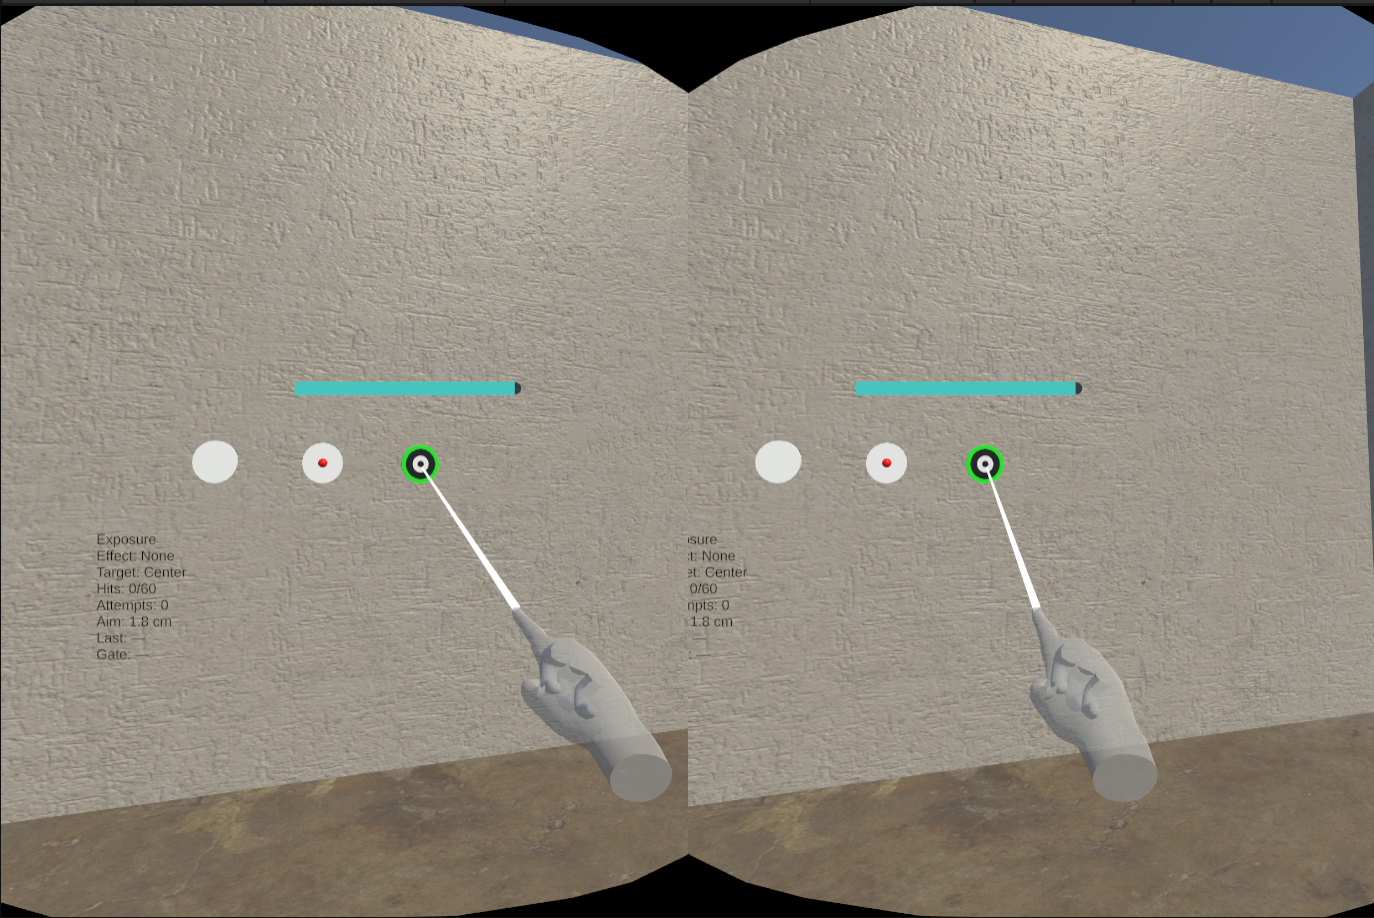
\includegraphics[width=0.88\linewidth]{img/3_Implementation/EmbodyDefaultWithLoading.png}
    \caption{Embodied interaction with the progress bar visible. The screenshot shows the exposure view in hand-tracking mode: the embodied hand representation replaces the controller model, the ray/debug line makes the pointing direction legible in the report, the active target still carries the bullseye cue, and the horizontal bar above the target wall visualizes the short loading or transition interval between accepted responses. Confirmation itself is handled by the non-dominant-hand controller trigger.}
    \label{fig:unity-embodied-loading}
\end{figure}

The Unity scene was intentionally kept sparse so that the experimental variables stayed legible. The participant stands in front of one target wall inside a narrow room, and the tasks are then expressed by changing what appears on that wall rather than by changing the surrounding environment. This means that the same physical setup can support Open-Loop Pointing, Line Bisection, Landmark, and Exposure without introducing large scene changes between phases. The room, target plane, and controller or hand representation therefore work as a stable spatial frame for the whole baseline--exposure--post-exposure sequence.

\begin{figure}[H]
    \centering
    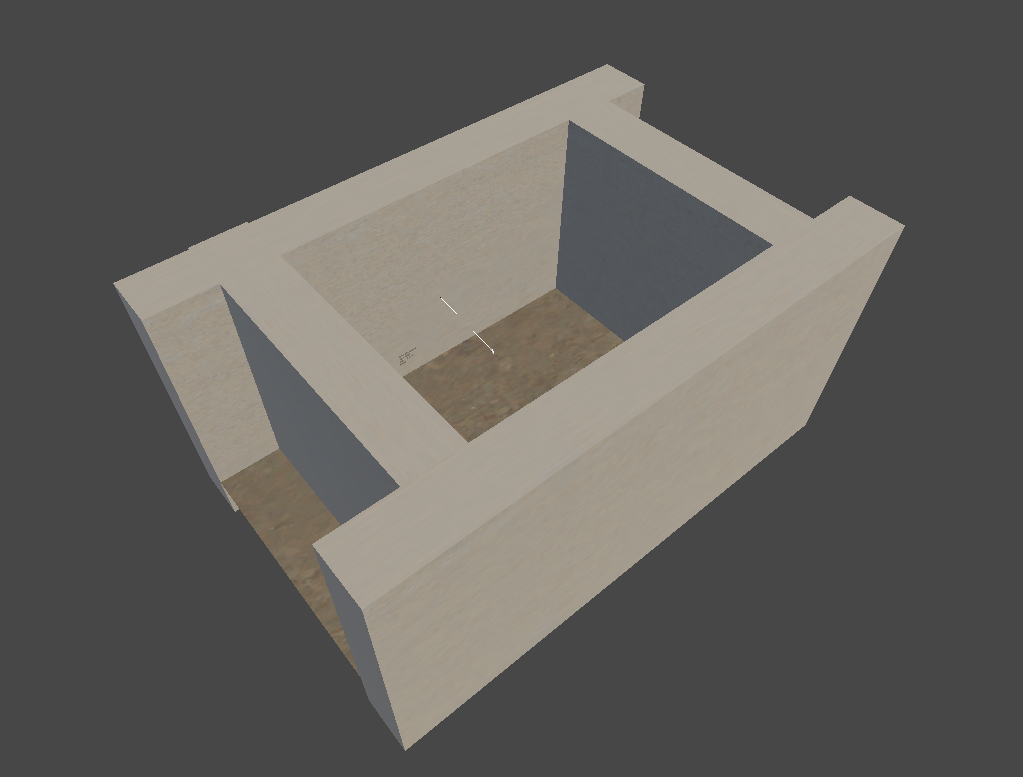
\includegraphics[width=0.78\linewidth]{img/3_Implementation/FullView.png}
    \caption{Overall Unity scene used by the prototype. The environment is deliberately minimal: one enclosed room, one target wall, and a constrained interaction area in front of that wall. This keeps the participant's spatial reference frame stable across tasks and makes the task-specific changes easy to attribute to the active task or effect rather than to a changing environment.}
    \label{fig:unity-overall-scene}
\end{figure}

The main configuration surface for these combinations is the \texttt{SandboxRunner.cs} Inspector. Rather than hard-coding a separate scene variant for each experiment condition, the runner exposes the main experimental switches in one place. The first Inspector screenshot in Figure~\ref{fig:unity-sandboxrunner-inspector} shows the top-level configuration categories: effect mode, task mode, scene references, XR input mode, active hand, controller-confirmation mitigation, task-transition timing, and calibration references. The second screenshot continues with the effect-specific parameters and flow controls: translation offset, rotation angle and axis, skew units/value/reference distance, experiment start and restart keys, automatic progression, play-mode stop behaviour, and debug-ray options. This is what makes the prototype a sandbox rather than a single-purpose scene, because the same runtime can be reconfigured into multiple task/effect/input combinations from one component.

\begin{figure}[H]
    \centering
    \begin{minipage}[t]{0.49\linewidth}
        \centering
        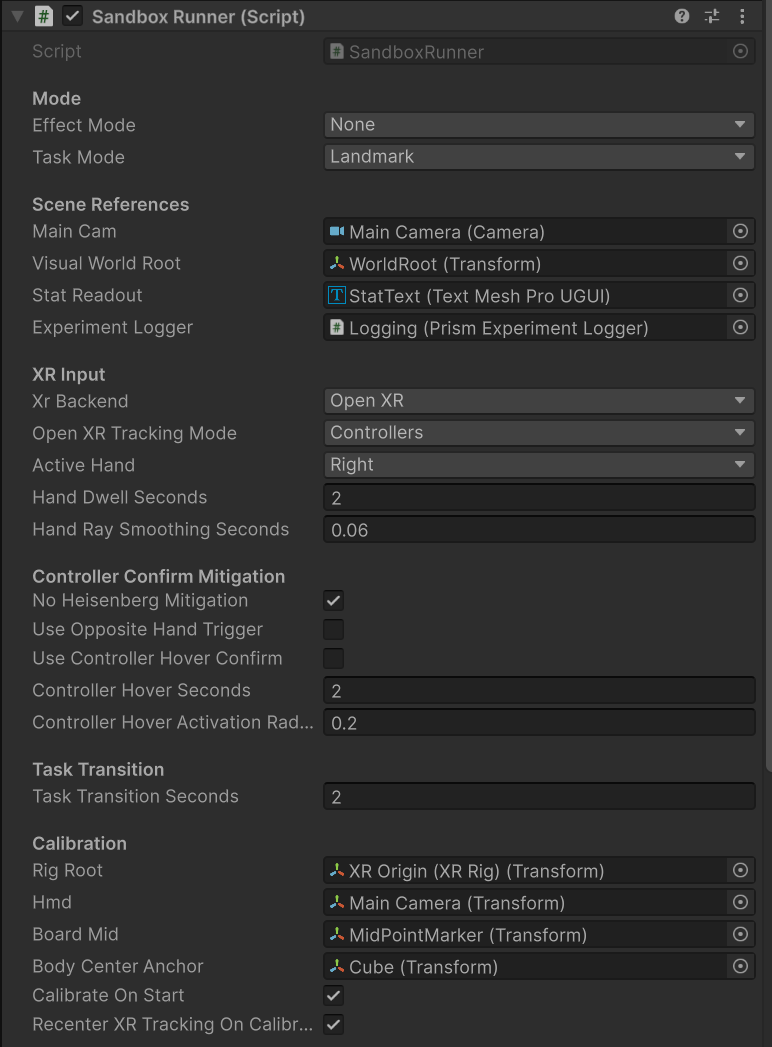
\includegraphics[width=\linewidth]{img/3_Implementation/BaseInspector.png}
    \end{minipage}\hfill
    \begin{minipage}[t]{0.49\linewidth}
        \centering
        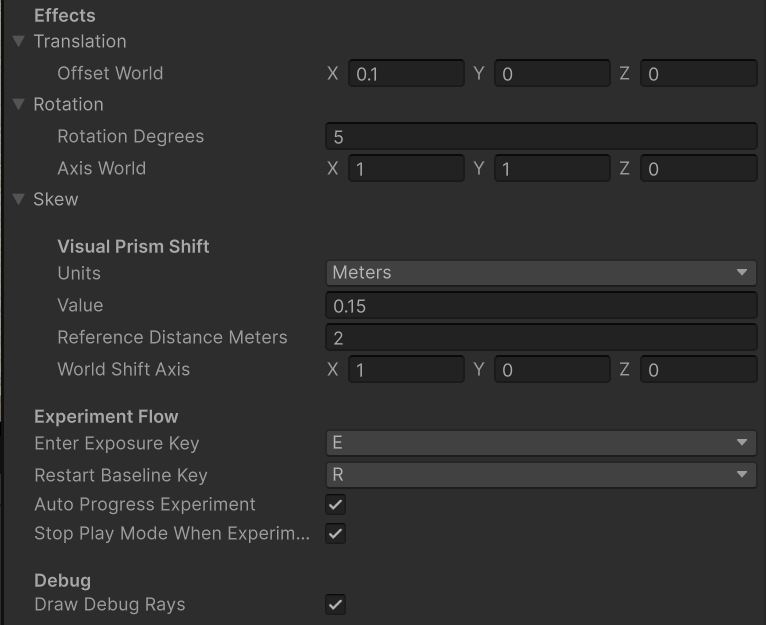
\includegraphics[width=\linewidth]{img/3_Implementation/EffectAndDebugInspector.png}
    \end{minipage}
    \caption{\texttt{SandboxRunner.cs} Inspector views. Left: the base runtime configuration, including task and effect selection, scene references, XR backend and tracking mode, active hand, confirmation-mitigation options, transition timing, and calibration anchors. Right: the effect and experiment-flow controls, including translation, rotation, and skew parameters together with automatic progression, restart behaviour, and debug options. Together, these views show how the implementation exposes the major experimental variables through one shared orchestration component.}
    \label{fig:unity-sandboxrunner-inspector}
\end{figure}

\subsection{Task-Specific Execution}
\label{subsec:implementation-tasks}

On top of the shared runtime sit the four task scripts: \texttt{OpenLoopPointingTask.cs}, \texttt{LineBisectionTask.cs}, \texttt{LandmarkTask.cs}, and \texttt{ExposureTask.cs}. All four consume the unified input supplied by \texttt{SandboxRunner.cs}, but each script still has to define its own display logic, response handling, and measurement output.

\texttt{OpenLoopPointingTask.cs} implements the simplest measurement task. The script creates one visible target, waits for the participant to adopt the required posture, records one confirmed response, and stores the signed endpoint deviation relative to the intended target centre. Its role is therefore to turn one accepted pointing response into a stable per-trial value that can later be compared between baseline and post-exposure blocks. \texttt{LineBisectionTask.cs} reuses much of the same structural logic, but replaces the point target with a displayed line. Here the response is interpreted relative to the line's true midpoint, so the main output becomes a signed midpoint deviation. \texttt{LandmarkTask.cs} differs more clearly from the other two: instead of pointing toward one location, the participant judges which of two line segments appears longer. The script therefore builds the split-line stimulus, randomizes which side is objectively longer, and stores the response as a left/right choice together with correctness.

\texttt{ExposureTask.cs} is implemented separately because it serves a different experimental purpose. Rather than isolating one accepted response, it drives repeated acquisition of targets under the currently active perturbation. The underlying layout is still a horizontal left--centre--right arrangement, but the script normally chooses the next target in randomized order while avoiding immediate repetition. Each confirmed attempt is judged as hit or miss, the number of successful hits is tracked, and the runner is notified when the exposure block is complete. This is also the file in which participant-facing feedback is most explicit: the active target highlight changes from attempt to attempt, the bullseye cue follows the selected target, and hit markers show where accepted responses landed. These cues are implemented here because they belong to the exposure task itself rather than to the shared runtime.

Across the four scripts, the shared part is not the stimulus but the way a trial is handled. Each task receives transformed input from \texttt{SandboxRunner.cs}, decides when a response has been accepted, and writes its result into the same logging structure. This keeps the task differences local to the task scripts while baseline, exposure, and post-exposure data remain directly comparable.

The task screenshots in Figures~\ref{fig:unity-openloop-views} and~\ref{fig:unity-measurement-task-views} make this local variation visible. All tasks reuse the same room, target wall, pointer representation, and status readout, but they change the wall stimulus and the response interpretation. In other words, the participant-facing scene remains stable while the task logic changes underneath it.

One clarification is important for reading these static Unity figures. Where visible aiming rays appear in the screenshots, they are used as debug representations so the current pointing direction is legible in the report. They should therefore be understood as explanatory visualization rather than as evidence that a visible debug ray is a required participant-facing element of the final runtime configuration.

\begin{figure}[H]
    \centering
    \begin{minipage}[t]{0.57\linewidth}
        \centering
        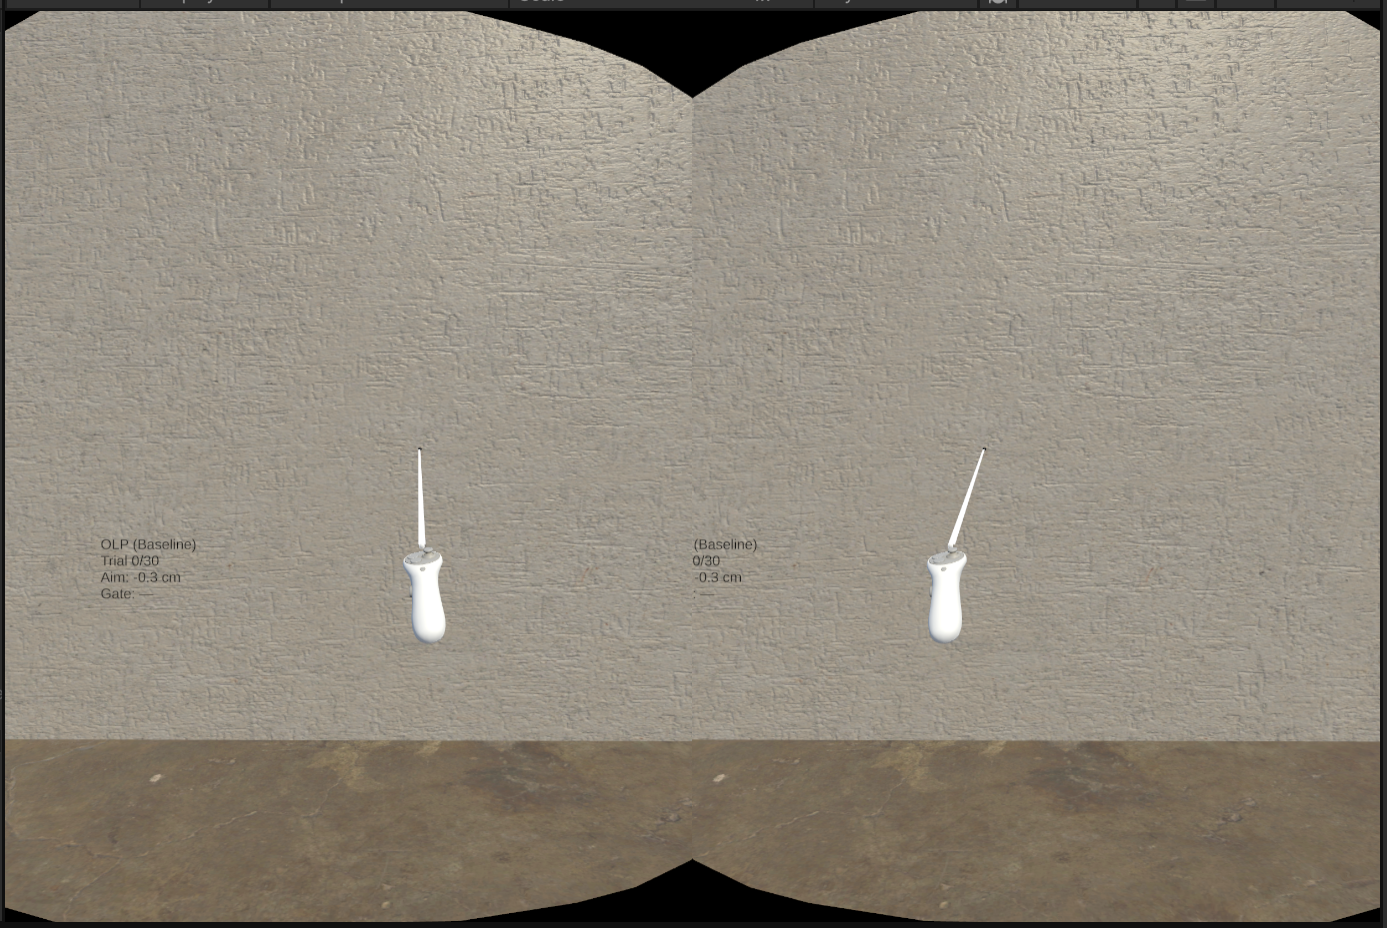
\includegraphics[width=\linewidth]{img/3_Implementation/OpenLoopFrontView.png}
    \end{minipage}\hfill
    \begin{minipage}[t]{0.40\linewidth}
        \centering
        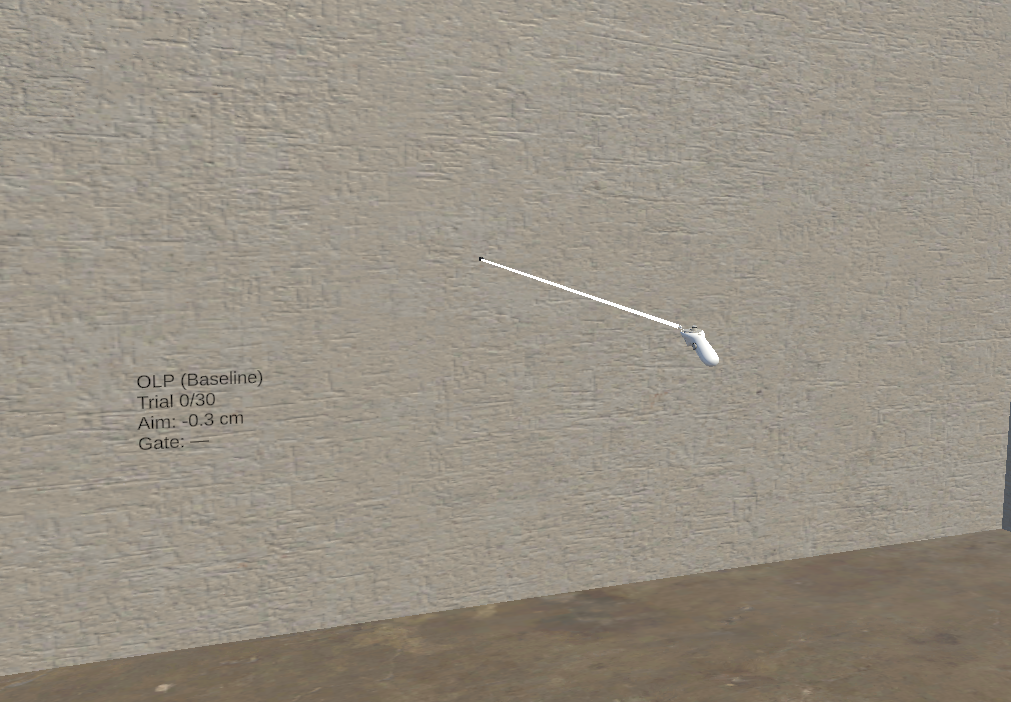
\includegraphics[width=\linewidth]{img/3_Implementation/OpenLoopBackView.png}
    \end{minipage}
    \caption{Open-Loop Pointing in Unity. Left: the stereoscopic task view, which keeps the visual presentation sparse and concentrates attention on the target wall, current pointing direction, and status readout. Right: an oblique scene view of the same task, which makes the wall-based pointing geometry easier to inspect from outside the headset view. Visible rays in these screenshots are documentation/debug representations of the aim direction rather than a required participant-facing element.}
    \label{fig:unity-openloop-views}
\end{figure}

\begin{figure}[H]
    \centering
    \begin{minipage}[t]{0.49\linewidth}
        \centering
        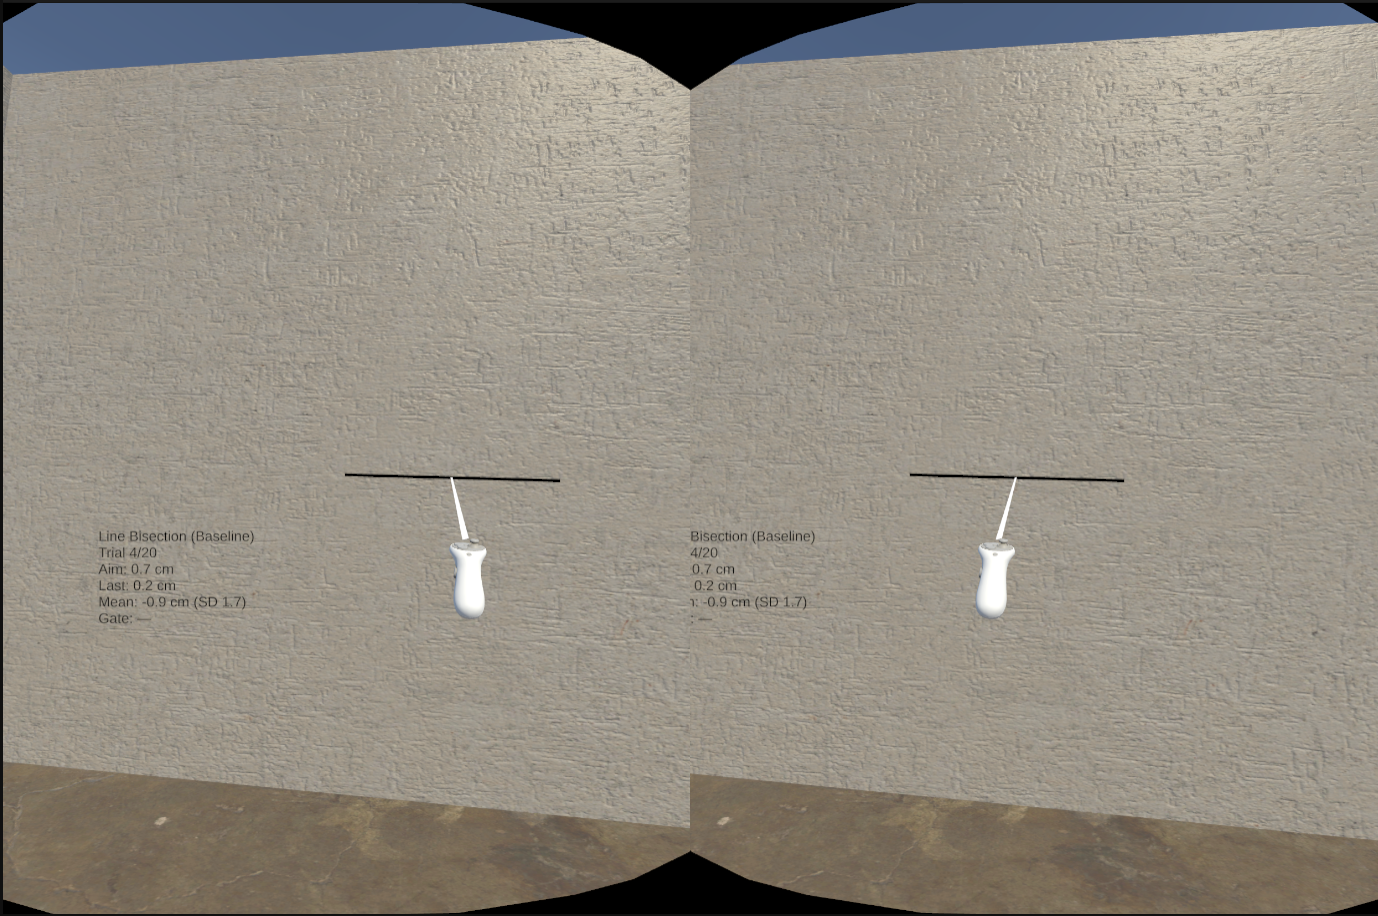
\includegraphics[width=\linewidth]{img/3_Implementation/LineBisection.png}
    \end{minipage}\hfill
    \begin{minipage}[t]{0.49\linewidth}
        \centering
        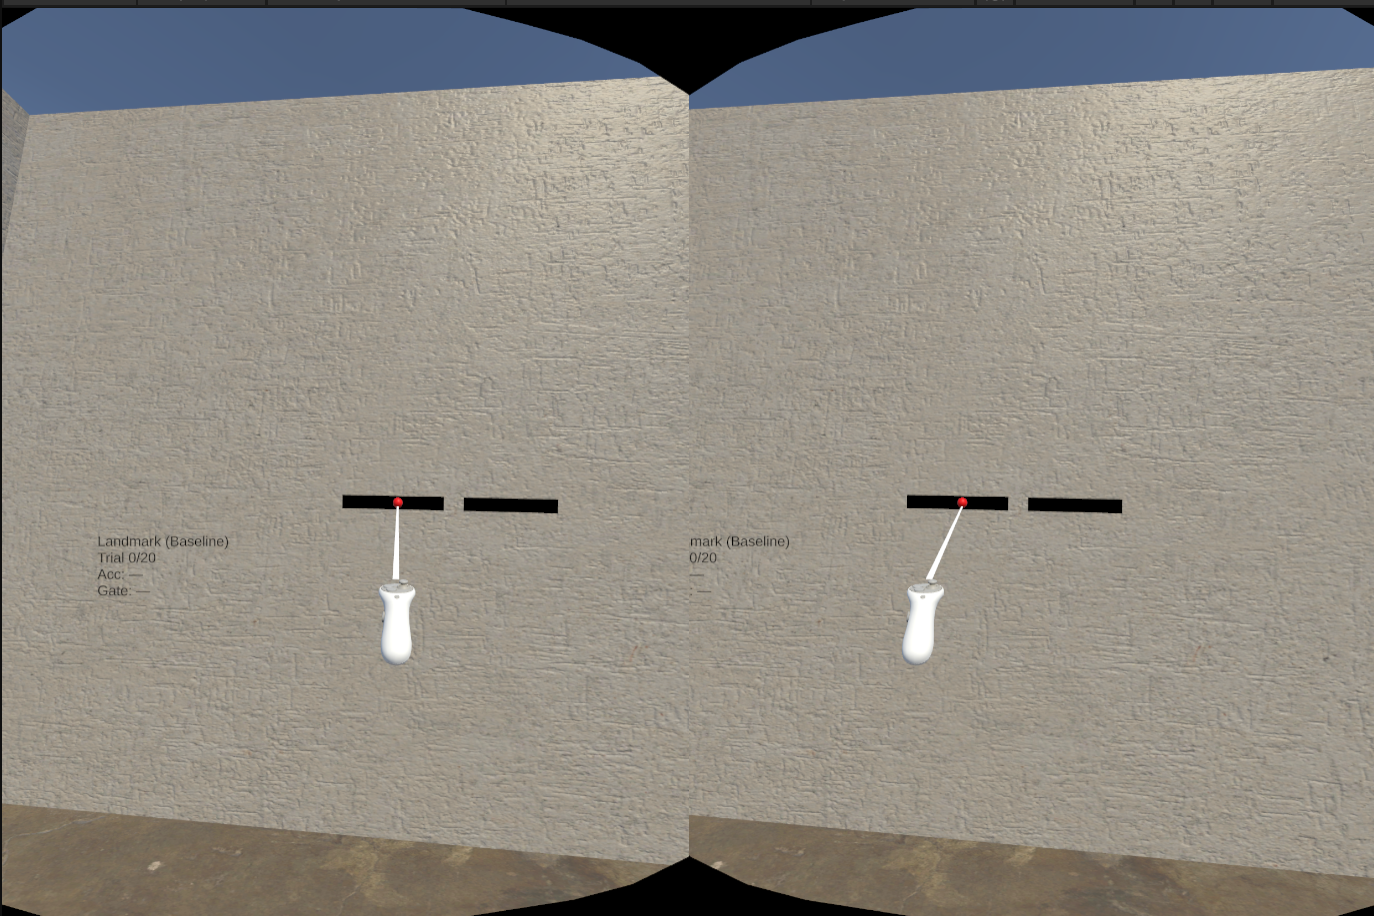
\includegraphics[width=\linewidth]{img/3_Implementation/Landmark.png}
    \end{minipage}
    \caption{Measurement-task implementations that reuse the same wall setup in different ways. Left: Line Bisection, where a horizontal line is shown on the wall and the response is interpreted relative to its true midpoint. Right: Landmark, where the wall instead presents two line segments separated by a gap and the participant makes a comparative left/right judgment. The implementation difference is therefore visible directly in the stimulus layout: one task asks for midpoint estimation, the other for comparative perceptual judgment.}
    \label{fig:unity-measurement-task-views}
\end{figure}

Exposure is where the runtime-side effect variations become most visible, because the repeated target-acquisition structure stays the same while the perturbation changes. Translation applies a fixed world-space offset to the transformed pointer representation. Rotation keeps the pose origin but rotates the pointing direction around the chosen axis. Skew is the most prism-like of the three in visual terms: it shifts the visible representation and the corresponding aim used for interaction so that the participant acts through a displaced hand or controller. The screenshots in Figure~\ref{fig:unity-exposure-effect-views} therefore matter because they show the same exposure grammar under different perturbation classes rather than four unrelated scenes.

\begin{figure}[H]
    \centering
    \begin{minipage}[t]{0.49\linewidth}
        \centering
        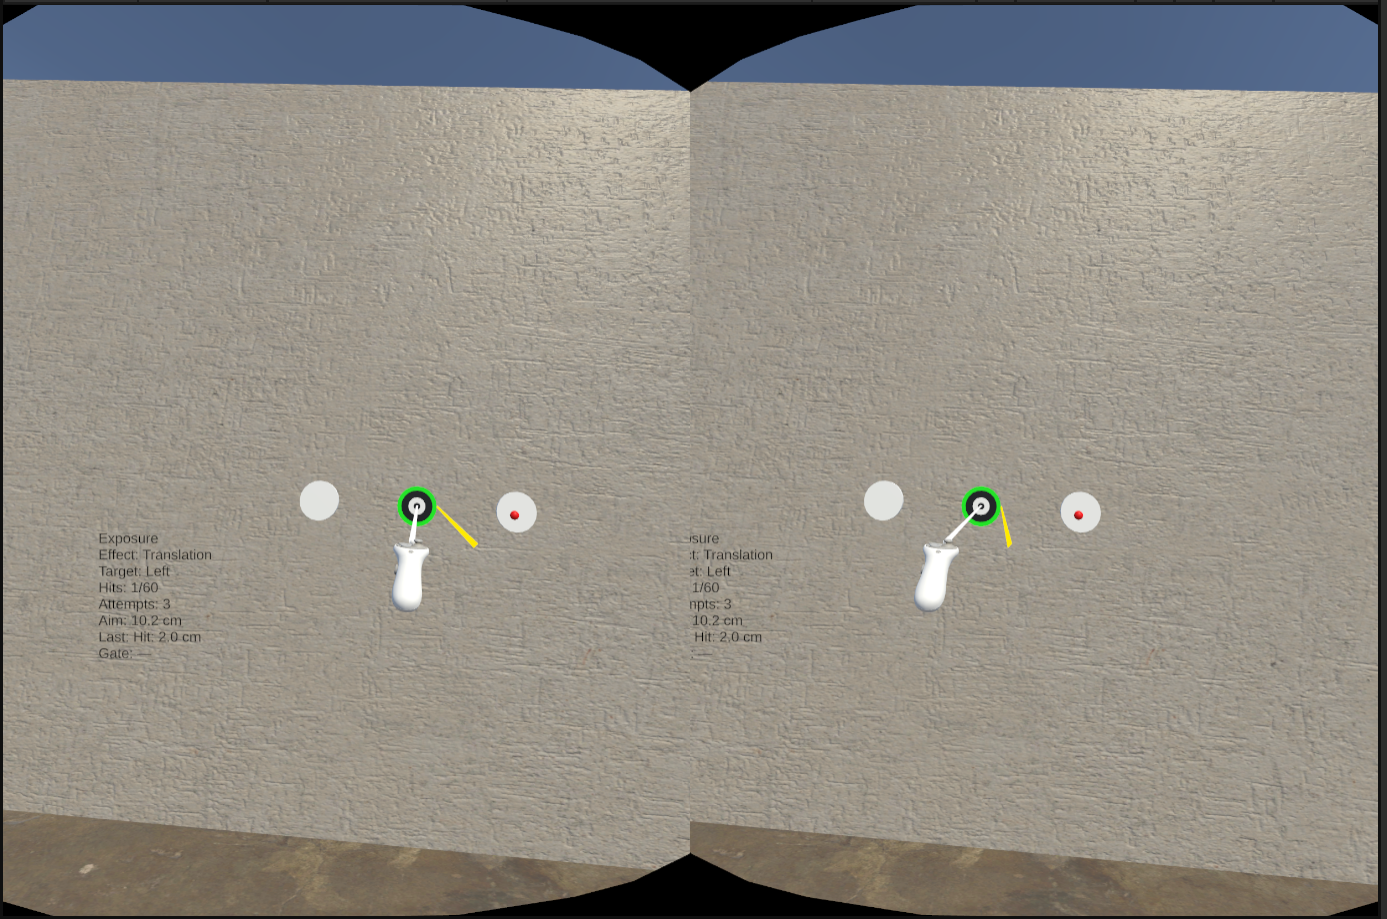
\includegraphics[width=\linewidth]{img/3_Implementation/ExposureTranslation1.png}
    \end{minipage}\hfill
    \begin{minipage}[t]{0.49\linewidth}
        \centering
        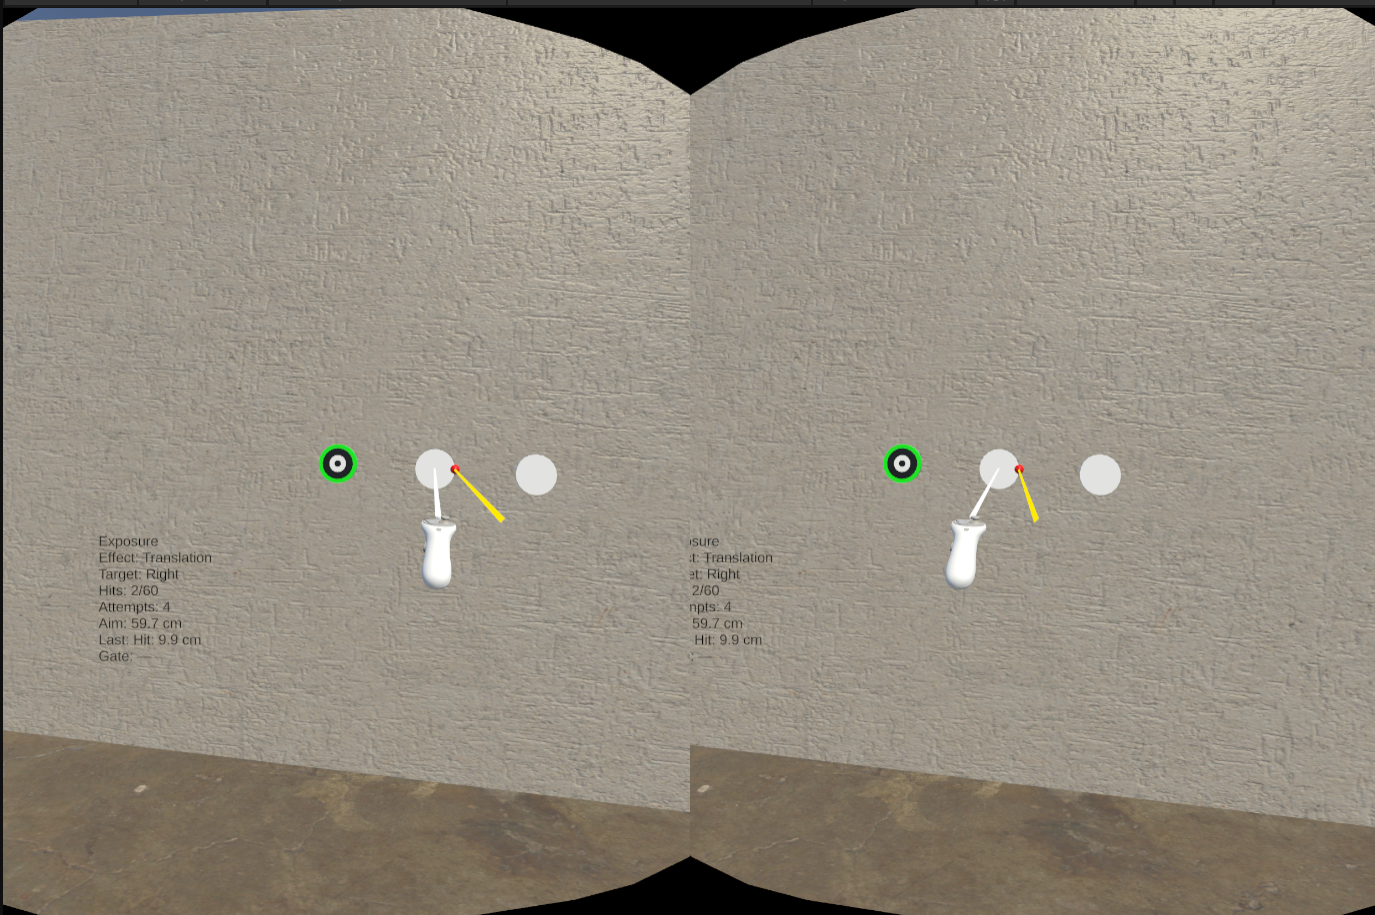
\includegraphics[width=\linewidth]{img/3_Implementation/ExposureTranslation2.png}
    \end{minipage}

    \medskip

    \begin{minipage}[t]{0.49\linewidth}
        \centering
        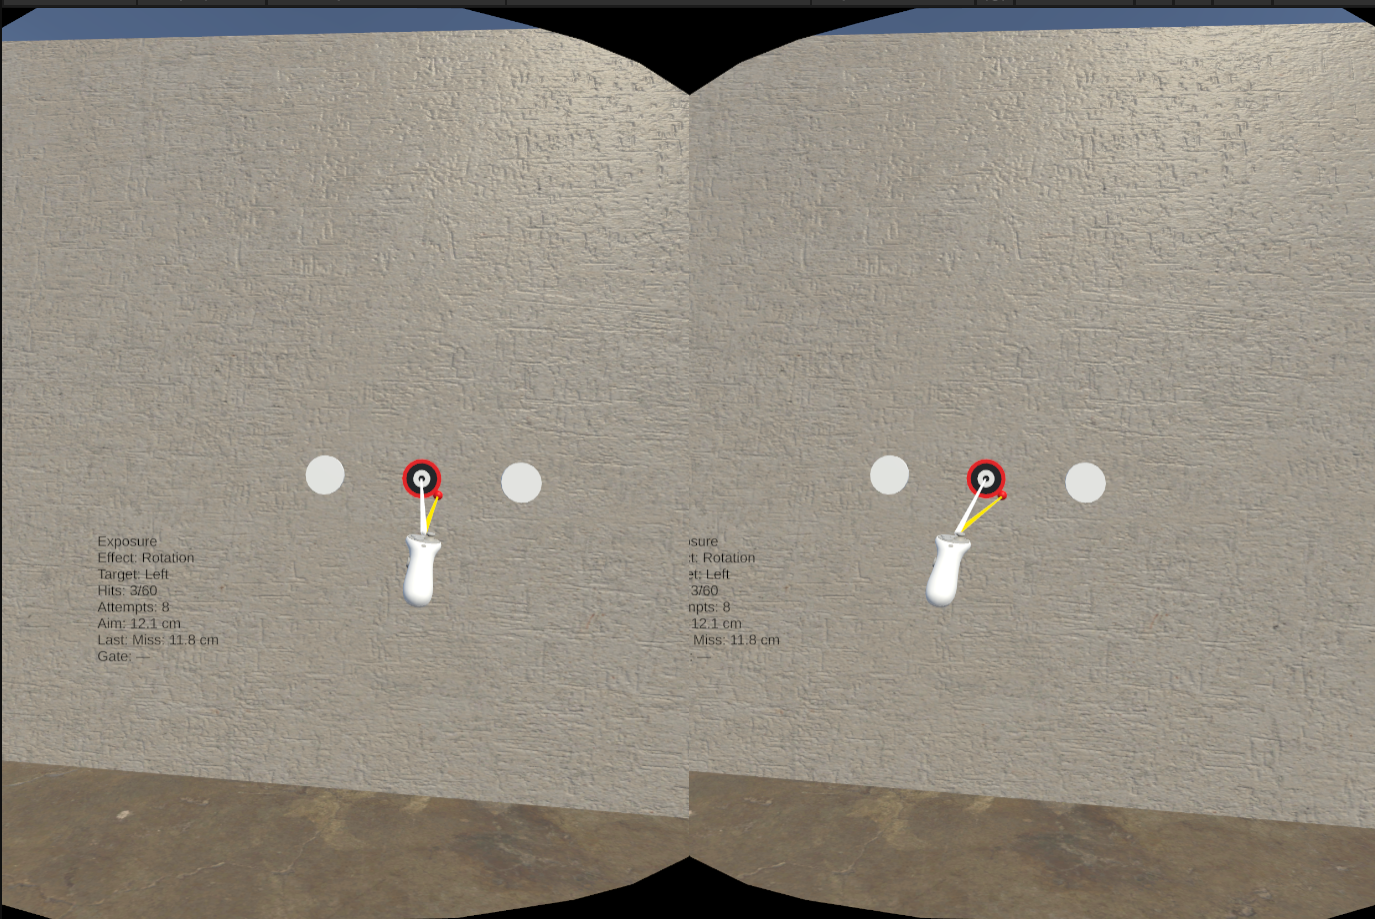
\includegraphics[width=\linewidth]{img/3_Implementation/ExposureRotate.png}
    \end{minipage}\hfill
    \begin{minipage}[t]{0.49\linewidth}
        \centering
        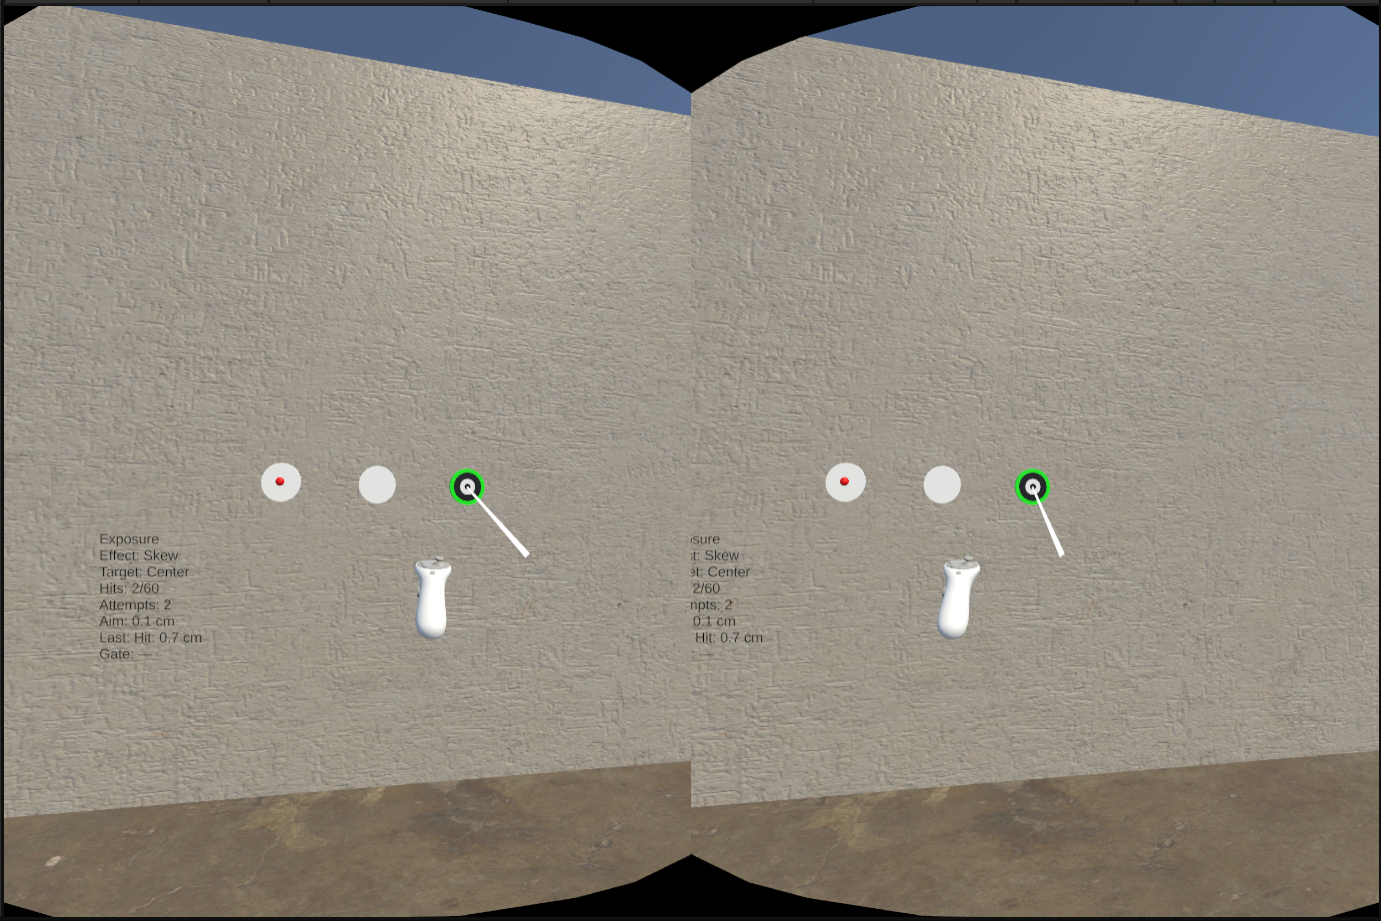
\includegraphics[width=\linewidth]{img/3_Implementation/ExposureSkew.png}
    \end{minipage}
    \caption{Exposure phase under the implemented perturbation types. Top left and top right: two moments from the translation condition, included to show that the repeated three-target layout stays fixed while the active target, bullseye cue, and hit marker update from attempt to attempt. Bottom left: the rotation condition, where the target layout remains the same but the pointing direction is rotated relative to the target wall. Bottom right: the skew condition, which behaves as a visual prism-style shift by displacing the visible hand or controller representation and its corresponding aim. Across all four screenshots, the same exposure structure remains visible: three horizontally arranged targets, one highlighted active target, a bullseye cue on that selected target, an aim/debug line for documentation, the last registered hit location, and the status readout on the left.}
    \label{fig:unity-exposure-effect-views}
\end{figure}

\subsection{Logging as the Bridge Between Unity and Analysis}
\label{subsec:implementation-logging}

The main implementation bridge between Unity and the later analysis is the custom Prism logging layer. Two project-specific scripts were created for this purpose: \texttt{PrismExperimentLogger.cs} and \texttt{PrismSampleLogger.cs}. Both extend the inherited \texttt{LoggingManager} from the Whack-a-Mole codebase, so the prototype reuses an existing session-logging structure instead of replacing it, but each logger adds prism-specific information for a different analytical purpose.

\texttt{PrismExperimentLogger.cs} writes the discrete structure of the run. It stores session metadata, block transitions, accepted measurement trials, exposure attempts, target spawns, exposure completion, and block- or task-level summaries. It also decides whether a session should count as \emph{Finished} or \emph{Aborted}, based on whether the participant actually passed through baseline, exposure, and post-exposure. In practice, this means that each accepted response can later be located in the correct phase, task, effect mode, input mode, and confirmation condition.

\texttt{PrismSampleLogger.cs}, by contrast, writes the continuous time series. At a fixed sampling rate it stores the transformed pointer together with the main pose and task-state information needed to reconstruct movement traces. These rows make it possible to inspect approach trajectories and later derive movement-phase measures such as acceleration, deceleration, or hover when needed. Table~\ref{tab:prism-logger-split} summarizes the division of responsibility between the two logging scripts.

This logging architecture is also where the project's concern for consistency becomes most concrete. The same run is represented in four collections --- \texttt{Meta}, \texttt{Event}, \texttt{Sample}, and \texttt{Summary} --- and each collection contributes a different perspective on the same session. By keeping the field names and block/task labels stable across these collections, the implementation makes it possible to inspect the same run as event summaries, quality checks, or movement traces without writing a different loader for every task and every effect.

\begin{table}[H]
    \centering
    \footnotesize
    \setlength{\tabcolsep}{5pt}
    \renewcommand{\arraystretch}{1.18}
    \begin{tabularx}{\linewidth}{|
        >{\raggedright\arraybackslash}p{0.25\linewidth}|
        >{\raggedright\arraybackslash}X|
        >{\raggedright\arraybackslash}p{0.28\linewidth}|}
        \hline
        \textbf{Logger} & \textbf{Writes} & \textbf{Primary later use} \\
        \hline
        \texttt{PrismExperimentLogger.cs} & Metadata, block transitions, accepted trials, exposure attempts, target spawns, completion states, and summary rows. & Session status, aftereffect summaries, block-level comparisons, and phase-aware filtering in the dashboard. \\
        \hline
        \texttt{PrismSampleLogger.cs} & Regular samples of transformed pointer state, head/controller poses, confirmation state, and current task context. & Trajectory reconstruction and later derivation of movement-phase measures such as acceleration, deceleration, and hover. \\
        \hline
    \end{tabularx}
    \caption{Division of responsibility between the two custom logging scripts.}
    \label{tab:prism-logger-split}
\end{table}

\subsection{RShiny Analysis Layer}
\label{subsec:implementation-rshiny}

The Unity screenshots above show what the participant and experimenter see during runtime; the analysis layer then reconstructs those same runs after they have been logged. The final project-specific script is \texttt{app.R}, which serves as the entry point to the local RShiny analysis dashboard. This file is the analysis-side counterpart to the Unity logging layer. The app first discovers completed sessions by grouping together the separate \texttt{Meta}, \texttt{Event}, \texttt{Sample}, and \texttt{Summary} CSV files belonging to the same session. It then loads the selected session and reorganizes the data into views that support inspection of the completed run. In practice, this means that the same raw logs can be viewed as single-session summaries, cross-session comparisons, quality checks, spatial hit distributions, or projected approach trajectories.

Within \texttt{app.R}, the logic is organized around a set of helper functions that each transform one part of the logging schema into a more interpretable view. Summary helpers reconstruct aftereffect interpretations from \texttt{Summary.csv}. Quality helpers turn accepted trials or exposure attempts into outlier counts, trend lines, and hit-rate summaries. Spatial helpers interpret event rows differently depending on whether the selected task is Open-Loop, Line Bisection, Landmark, or Exposure. Trajectory helpers combine \texttt{Event.csv} and \texttt{Sample.csv} so that one accepted exposure attempt can be reconstructed as a projected aim path on the target plane. The dashboard then reconnects these views to the currently selected session and task, so that the visible tables and plots change together when the user changes the selection.

The dashboard is organized into six tabs. \emph{Summary} focuses on one selected session and reconstructs the main aftereffect interpretation. \emph{Compare} moves to the cross-session level and asks how task, effect, and input mode differ across runs. \emph{Participant} summarizes the eight modules belonging to one participant so within-participant patterns can be inspected directly before collapsing data across participants. \emph{Quality} inspects block-level stability and unusually large errors within one task/block combination. \emph{Spatial} re-expresses accepted responses and exposure events as positions on the task plane. \emph{Trajectories} gives the most detailed inspection: for Exposure it shows projected approach behaviour toward the target plane, and for non-exposure tasks it reuses the same tab to show trial-by-trial signed and absolute response trends. The screenshots below make these analytical roles explicit.

These dashboard screenshots should be read as workflow demonstrations rather than as quantitative findings from the evaluation dataset. They are useful for showing what the analysis layer can reconstruct, but the evaluation results themselves are reported separately in Chapter~\ref{chap:results}.

\subsubsection{Summary View}

The Summary tab is the first pass over a completed session. It keeps the analysis at the single-session level and translates the \texttt{Aftereffect} rows in \texttt{Summary.csv} into a compact visual interpretation. The metric cards on the left answer the most immediate questions: which task was run, which effect was configured, how large the baseline-to-post signed change was, how large the unsigned aftereffect magnitude was, whether response spread increased or decreased, and how baseline and post averages compare directly. The plot on the right then turns that same summary row into a direct visual statement about aftereffect size. Below this view, the session summary table keeps the underlying summary rows visible so that the interpretation remains traceable back to the stored CSV fields rather than only to the explanatory cards.

\begin{figure}[H]
    \centering
    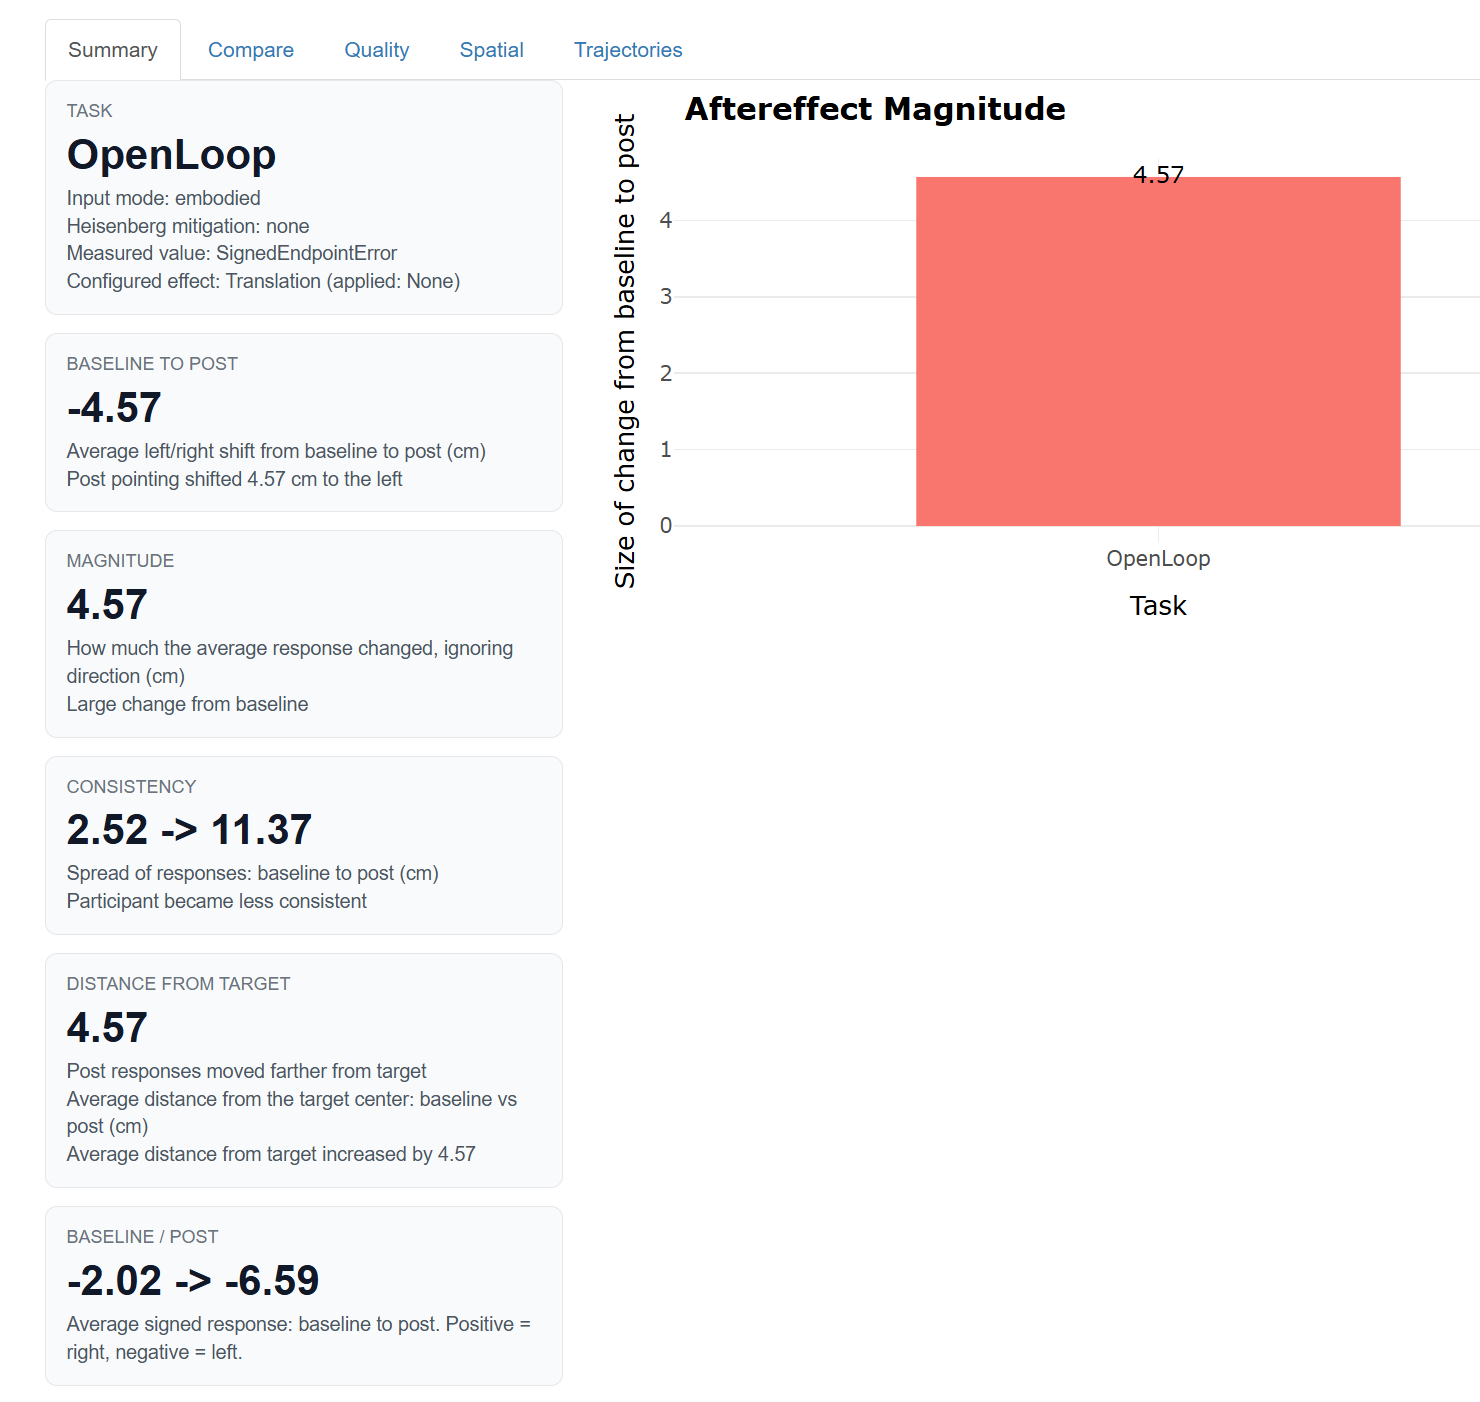
\includegraphics[width=0.95\linewidth]{img/3_Implementation/Summary.png}
    \caption{Summary tab for one selected session. The card column reconstructs the main aftereffect interpretation from \texttt{Summary.csv}: task identity, configured effect, signed baseline-to-post shift, unsigned magnitude, consistency change, distance-from-target interpretation, and the baseline/post averages themselves. The bar chart on the right provides the same result as a compact magnitude view, making it easy to see the size of change from baseline to post before moving on to the more detailed tabs.}
    \label{fig:rshiny-summary}
\end{figure}

\subsubsection{Compare View}

Where the Summary tab stays within one session, the Compare tab is designed for condition-level interpretation across many sessions. The filter row narrows the dataset by task, input mode, configured effect, and completion state. The card row then surfaces the most direct comparative answers: how many sessions are currently included, which task currently has the largest mean aftereffect, which exact task/effect/input-mode combination is strongest, and what the typical aftereffect magnitude looks like across the filtered subset. The main comparison plot emphasizes distribution rather than only averages, because the point spread and boxplots make it easier to see whether a condition looks stable, sparse, or highly variable. The tab also keeps the grouped statistics table and the per-session comparison table in view, so the reader can move from a visual condition pattern to the exact rows that generated it.

\begin{figure}[H]
    \centering
    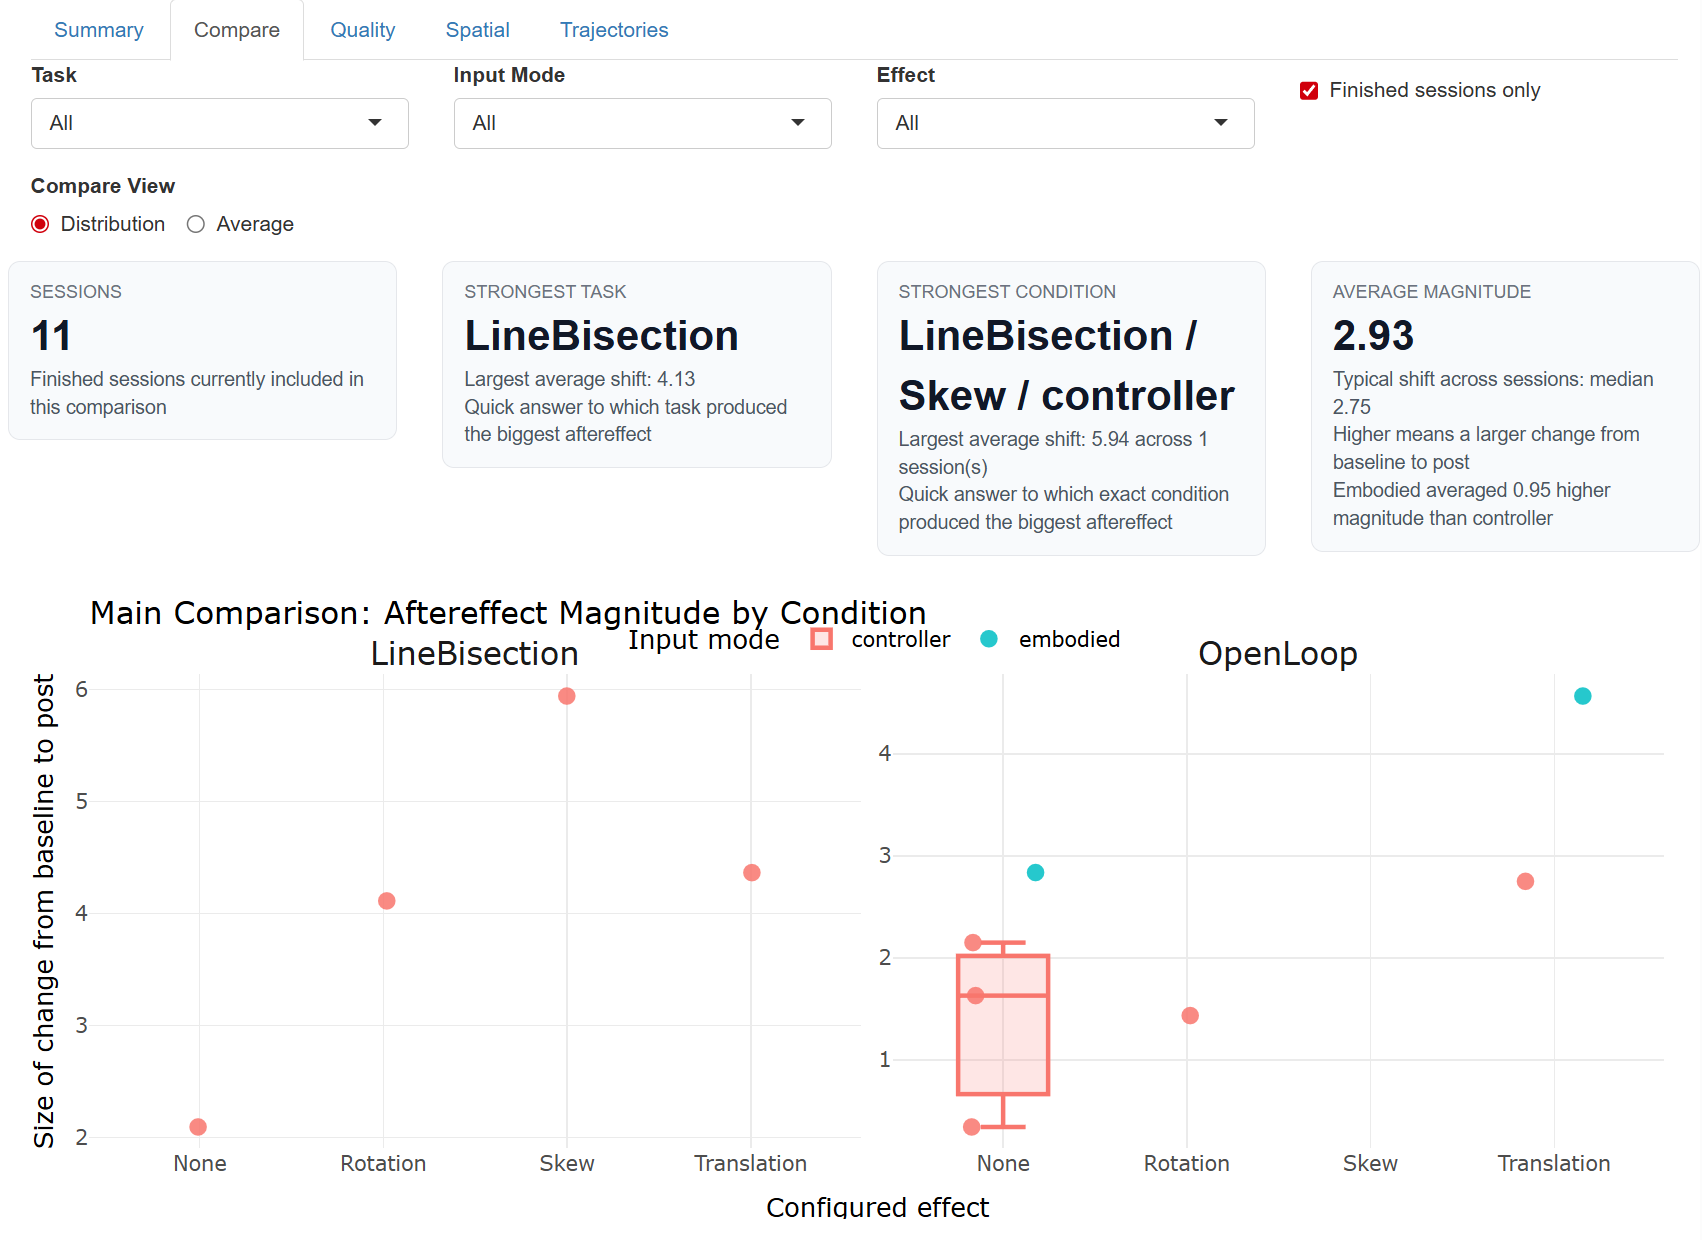
\includegraphics[width=0.98\linewidth]{img/3_Implementation/Compare1.png}
    \caption{Compare tab in its distribution view. The top controls filter the available sessions by task, input mode, effect, and whether only finished sessions should be retained. The card strip summarizes the currently filtered dataset, and the faceted comparison plot then shows aftereffect magnitude by configured effect while separating controller and embodied input. This is the dashboard's main cross-session visualization because it preserves both condition grouping and session-level spread.}
    \label{fig:rshiny-compare-distribution}
\end{figure}

\begin{figure}[H]
    \centering
    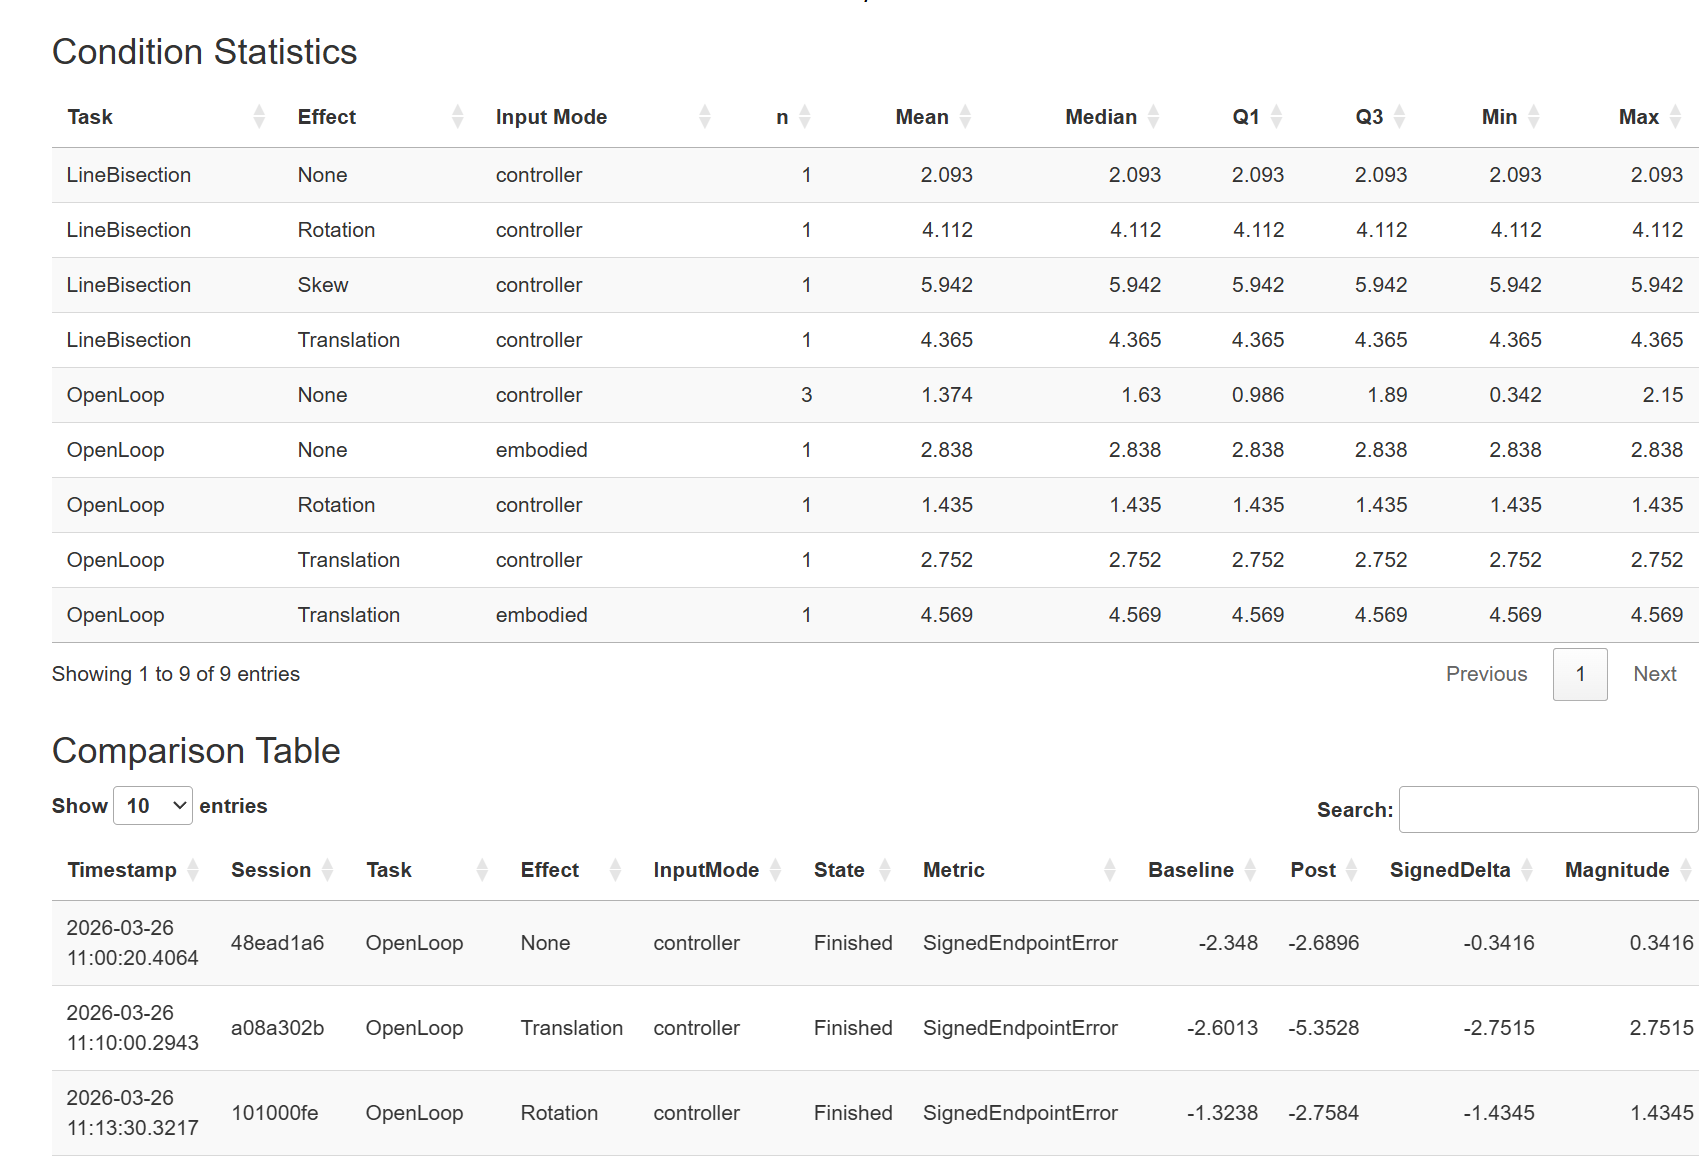
\includegraphics[width=0.98\linewidth]{img/3_Implementation/Compare2.png}
    \caption{Tabular part of the Compare view. The upper table groups sessions by task, effect, and input mode and reports descriptive statistics such as mean, median, quartiles, minimum, and maximum aftereffect magnitude. The lower table keeps the individual session rows visible, including timestamp, task, effect, input mode, baseline value, post value, signed delta, and magnitude. Together, these tables let the reader move from overview-level comparison back to the exact sessions that support a comparison claim.}
    \label{fig:rshiny-compare-tables}
\end{figure}

\subsubsection{Quality View}

The Quality tab inspects how stable one block was while it was being performed. Its purpose is not to estimate aftereffects directly, but to show whether the underlying trial sequence looks clean, noisy, improving, deteriorating, or dominated by a few unusually large deviations. The card column always reports the number of included trials or attempts, the mean absolute error, the number of unusually large errors, and the overall trend over the block. For Exposure, the tab also reports hit rate, because the outcome distinction between hits and misses is meaningful during the repeated target-acquisition phase. The plot itself is organized as a trial-by-trial error series with a linear trend line and a dashed outlier guide, so the reader can quickly see whether performance stayed stable or drifted as the block progressed.

\begin{figure}[H]
    \centering
    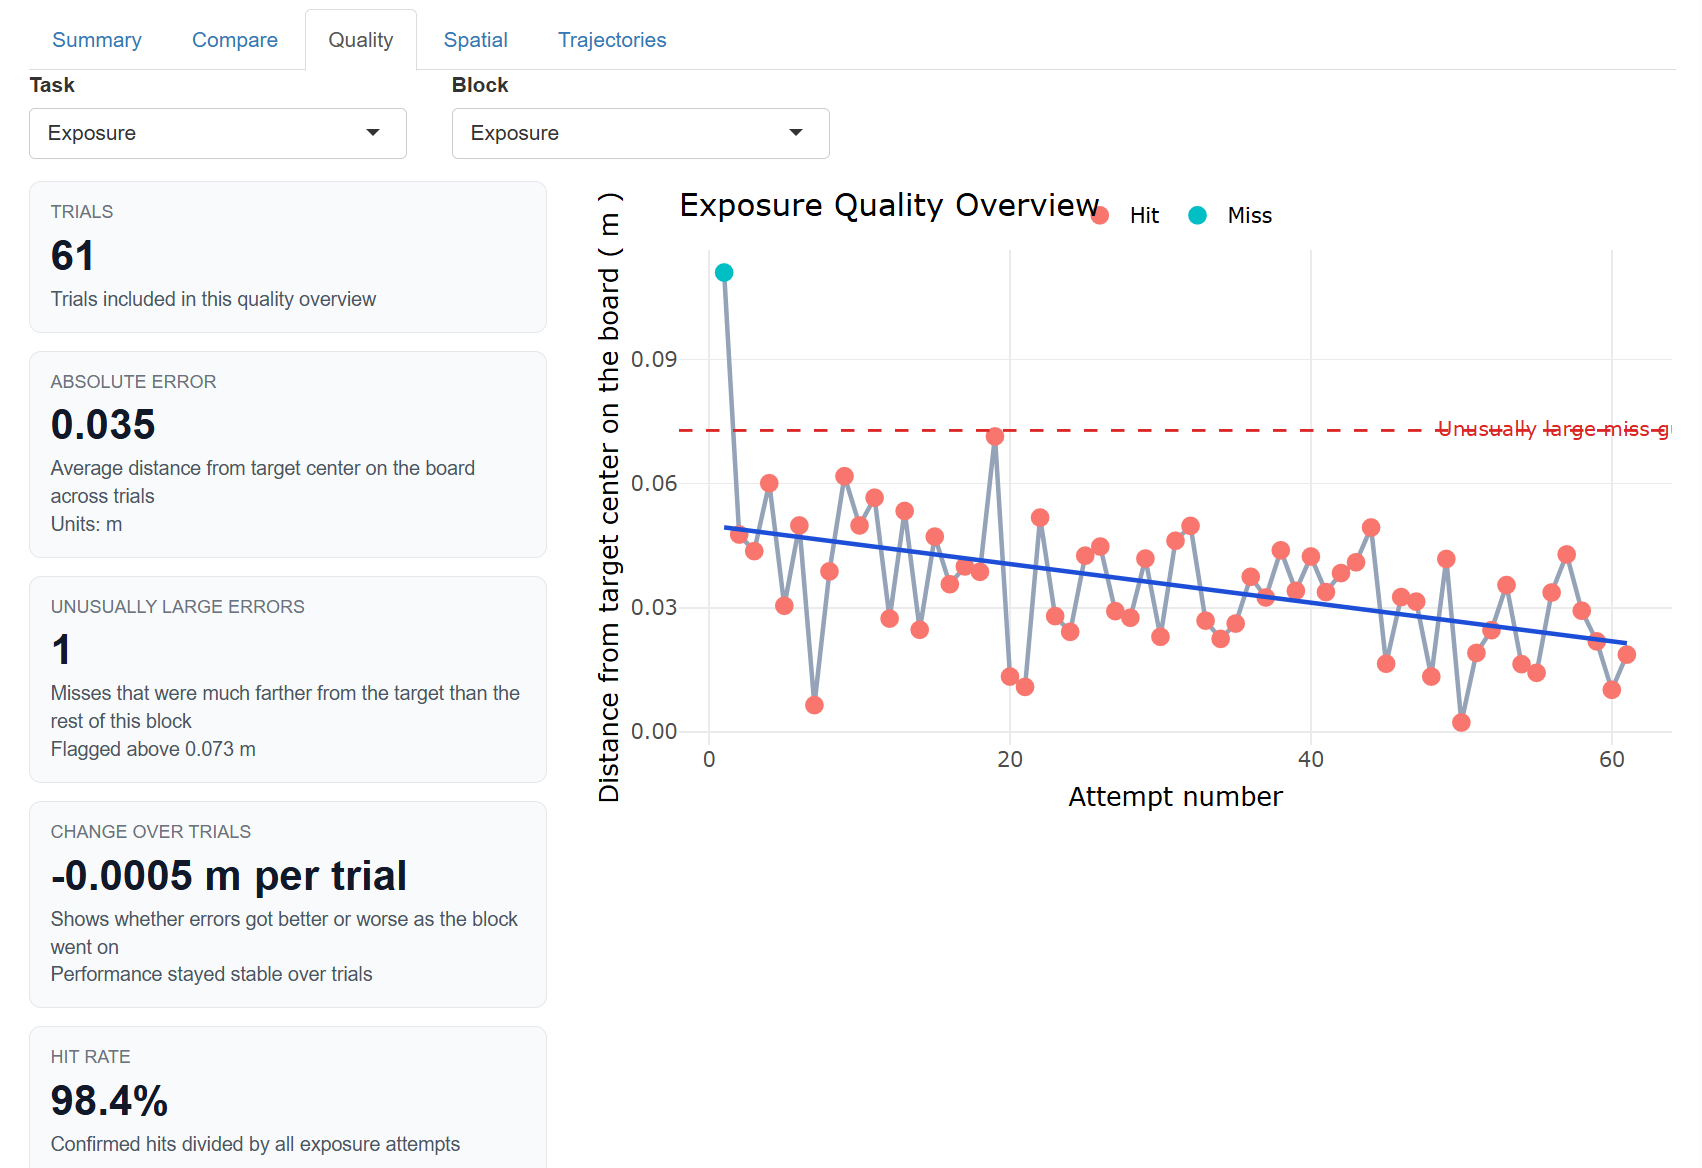
\includegraphics[width=0.98\linewidth]{img/3_Implementation/Quality1.png}
    \caption{Exposure example from the Quality tab. Each point is one exposure attempt, colored by hit or miss, and the vertical value is the final distance from target center on the board. The blue trend line shows whether distance from the target changed over attempts, while the red dashed line marks the threshold used for unusually large errors. The cards summarize how many attempts were included, the average absolute error, how many attempts exceeded the threshold, whether error drifted over time, and the hit rate for the block. This view is useful for deciding whether an exposure block looked stable enough to support later interpretation.}
    \label{fig:rshiny-quality-exposure}
\end{figure}

\begin{figure}[H]
    \centering
    \begin{minipage}[t]{0.49\linewidth}
        \centering
        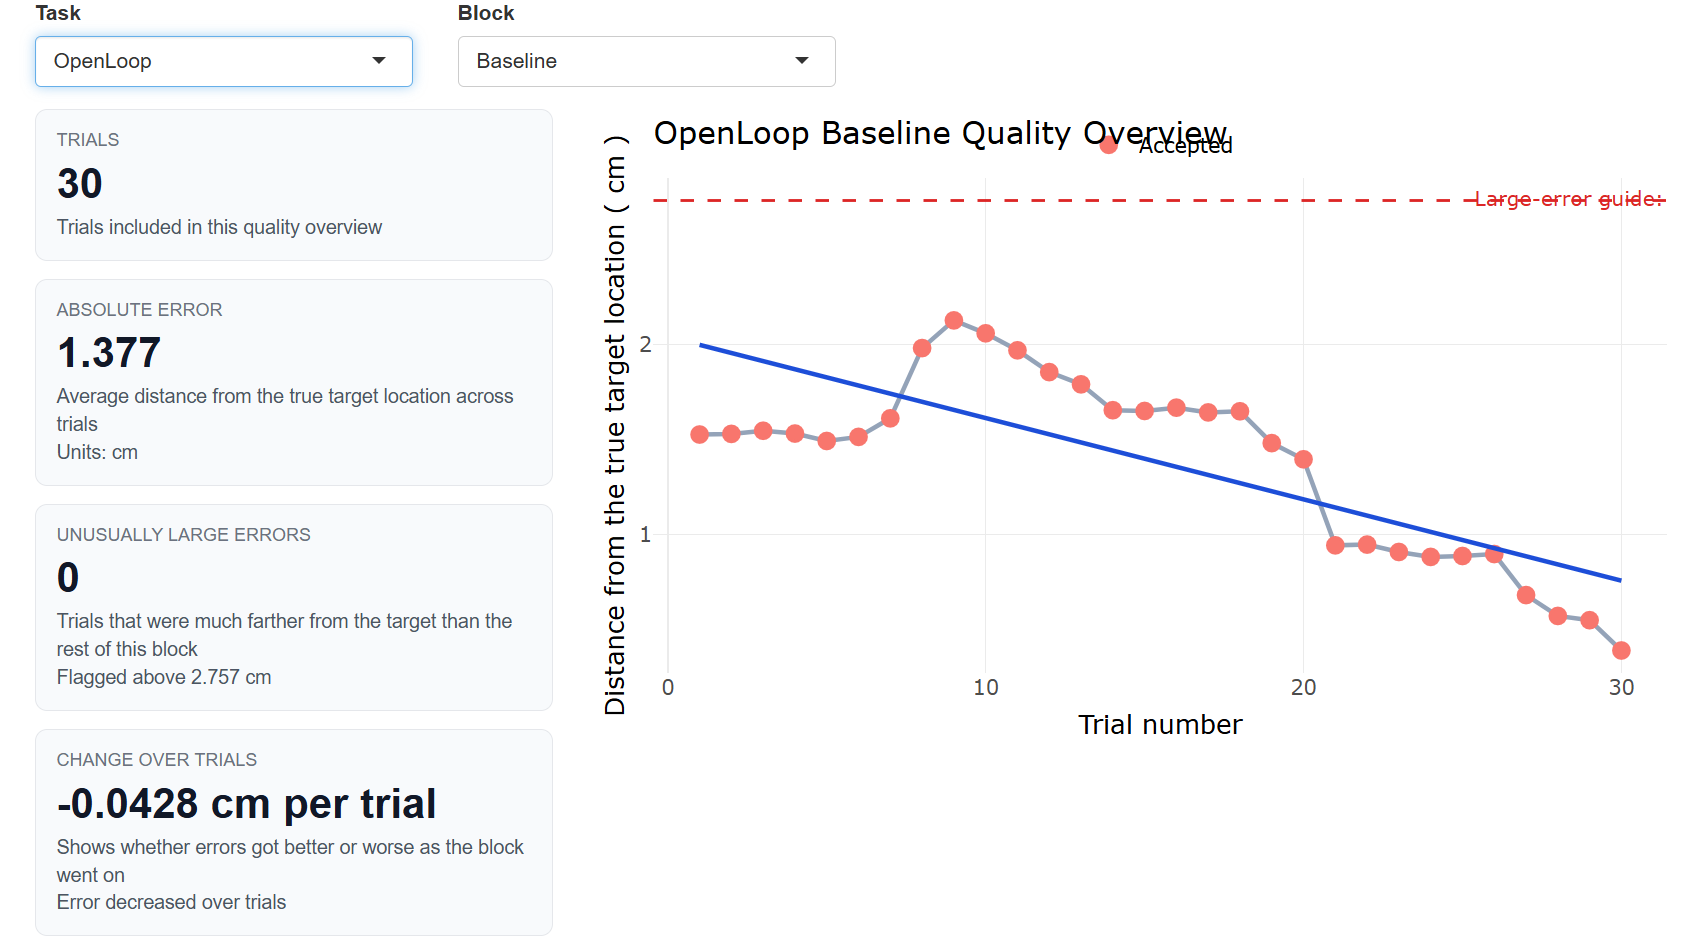
\includegraphics[width=\linewidth]{img/3_Implementation/Quality2.png}
    \end{minipage}\hfill
    \begin{minipage}[t]{0.49\linewidth}
        \centering
        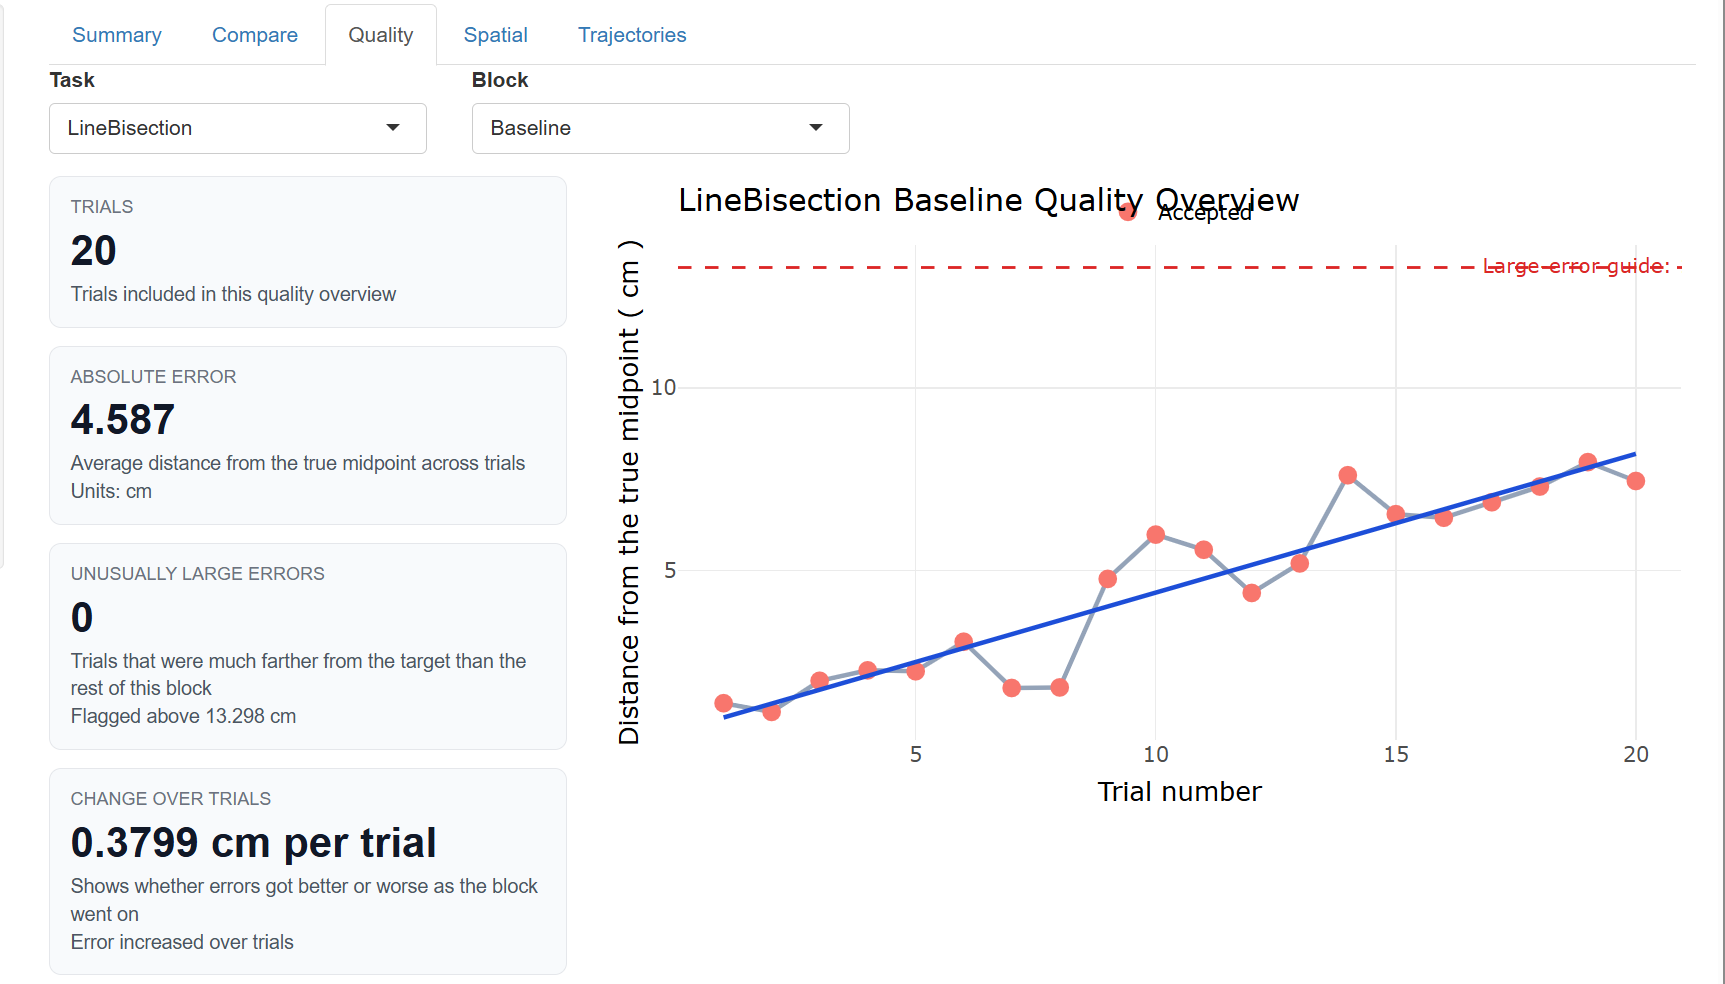
\includegraphics[width=\linewidth]{img/3_Implementation/Quality3.png}
    \end{minipage}
    \caption{Measurement-task examples from the Quality tab. Left: Open-Loop baseline quality, where each point is one accepted pointing response and the vertical value is absolute distance from the true target location. Right: Line Bisection baseline quality, where the same structure is reused but the error is measured relative to the true midpoint. These examples show that the tab keeps one shared quality grammar across tasks even though the error metric changes with the task definition.}
    \label{fig:rshiny-quality-measurement}
\end{figure}

\subsubsection{Spatial View}

The Spatial tab answers a different question from the Quality tab. Instead of focusing on trend over trial index, it asks where responses actually landed in space. For Exposure, that means preserving the two-dimensional task plane and plotting target positions together with hits and misses in board/world coordinates. For Open-Loop Pointing and Line Bisection, the same tab collapses the data to the spatial dimension that matters for the task: signed horizontal deviation from the true target center or from the true midpoint. This gives the reader a more literal view of leftward and rightward bias than the quality plots, which are oriented around distance and trend rather than spatial direction.

\begin{figure}[H]
    \centering
    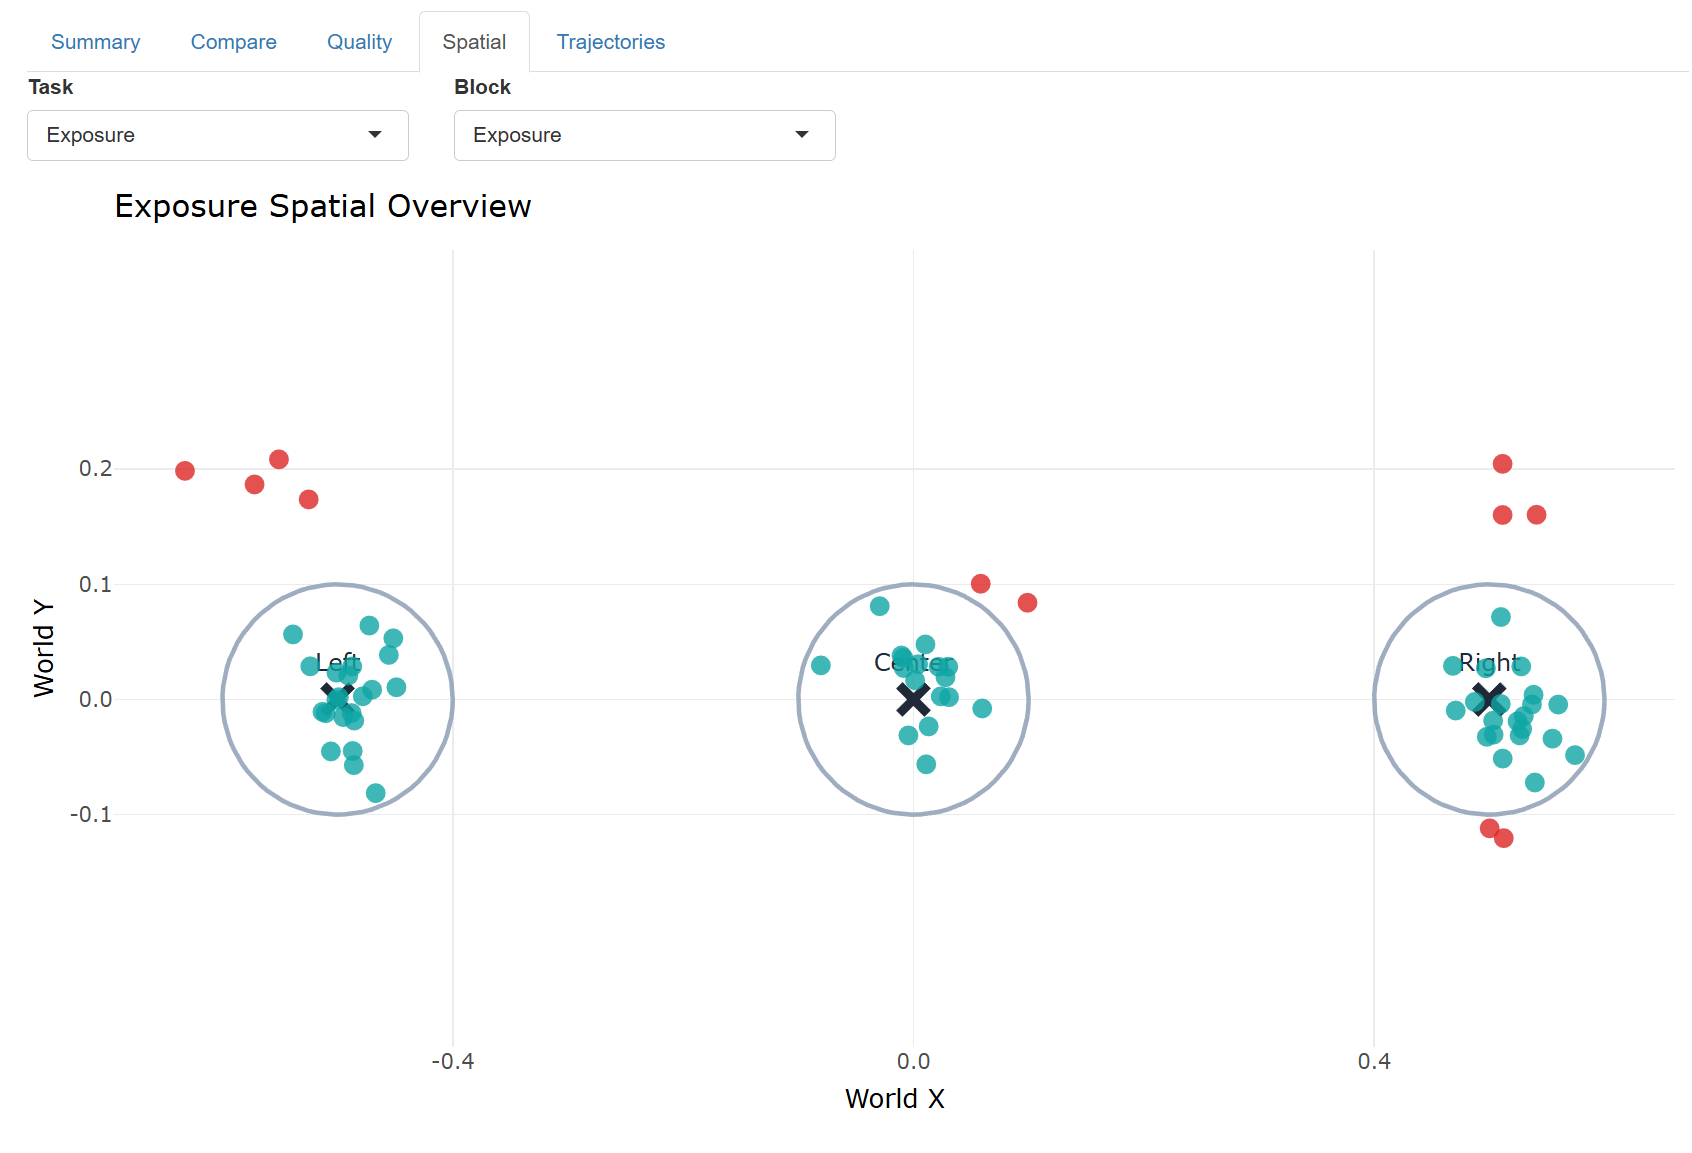
\includegraphics[width=0.98\linewidth]{img/3_Implementation/Spatial1.png}
    \caption{Exposure example from the Spatial tab. The crosses mark the left, centre, and right target centres, and the circular outlines show the target radius used to judge whether an attempt counted as a hit. Hits and misses are plotted around these targets in world space. This view makes it easy to see not only whether attempts succeeded, but also whether misses cluster above, below, or to one side of the left, centre, or right target.}
    \label{fig:rshiny-spatial-exposure}
\end{figure}

\begin{figure}[H]
    \centering
    \begin{minipage}[t]{0.49\linewidth}
        \centering
        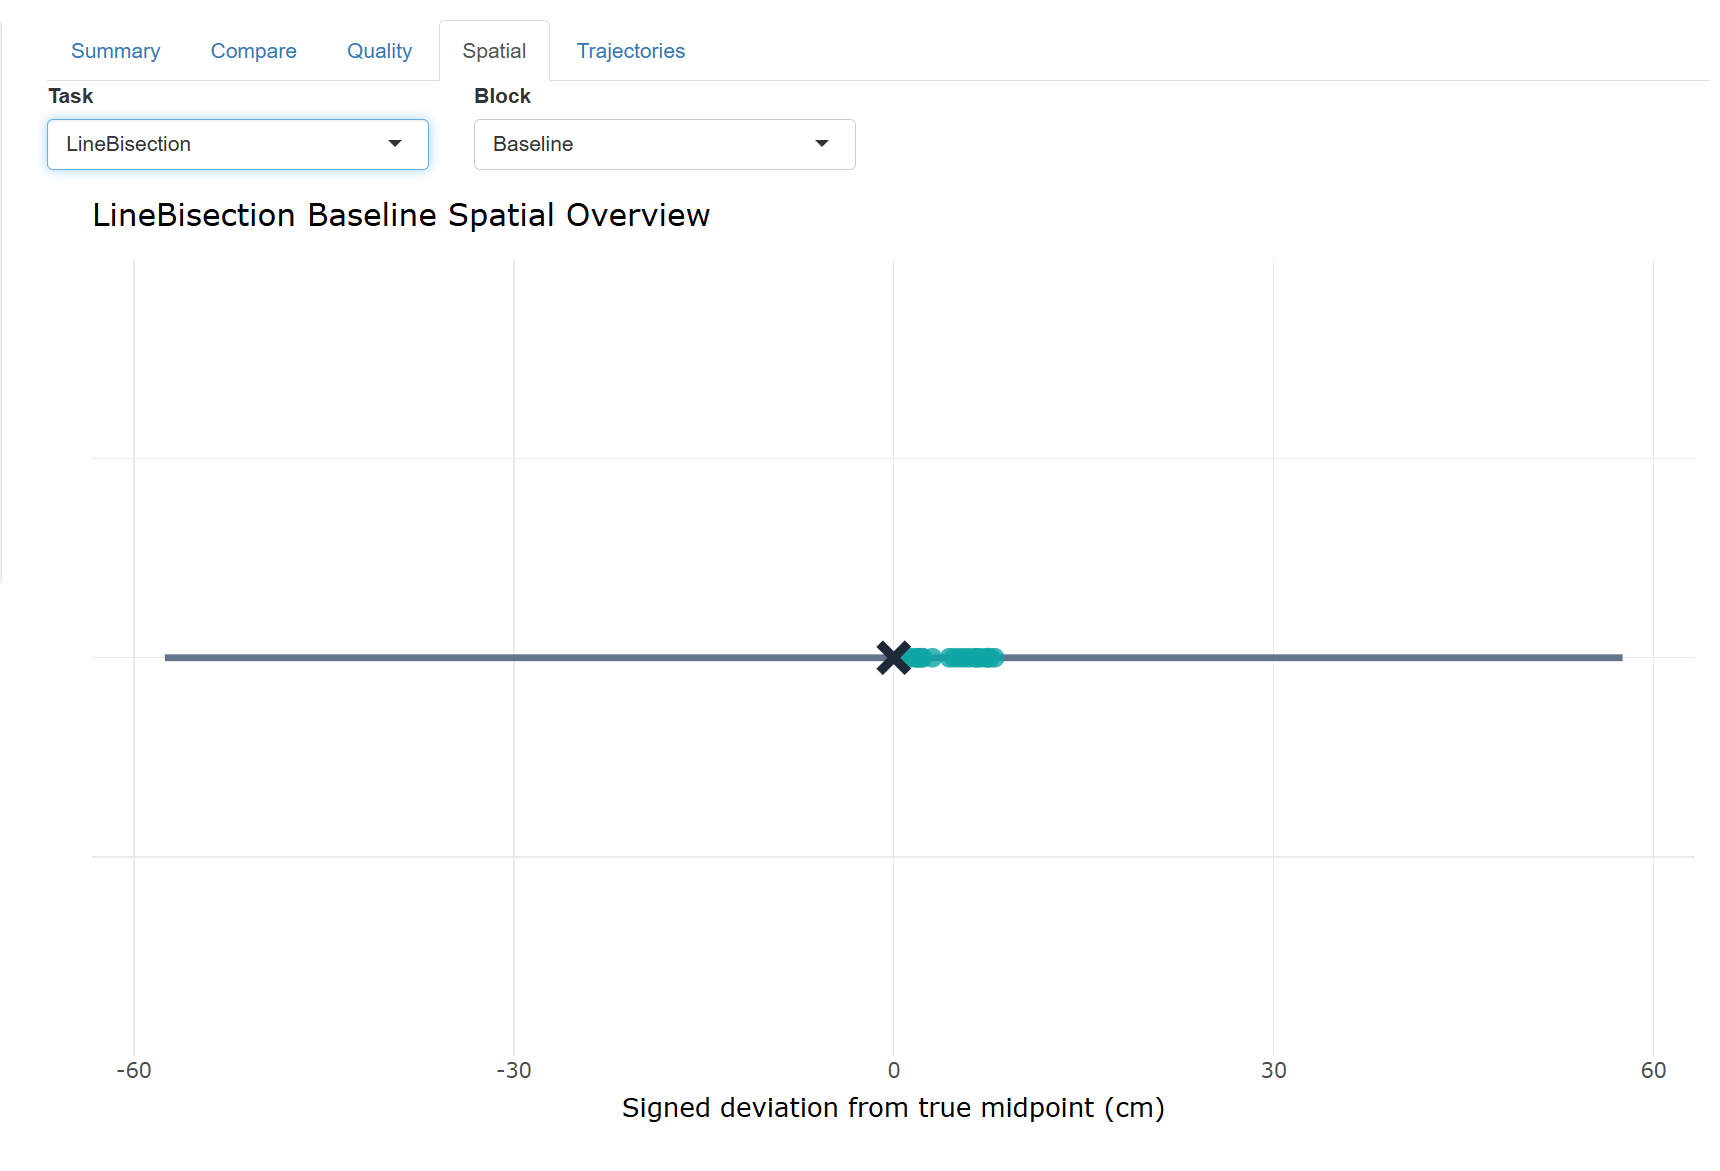
\includegraphics[width=\linewidth]{img/3_Implementation/Spatial2.png}
    \end{minipage}\hfill
    \begin{minipage}[t]{0.49\linewidth}
        \centering
        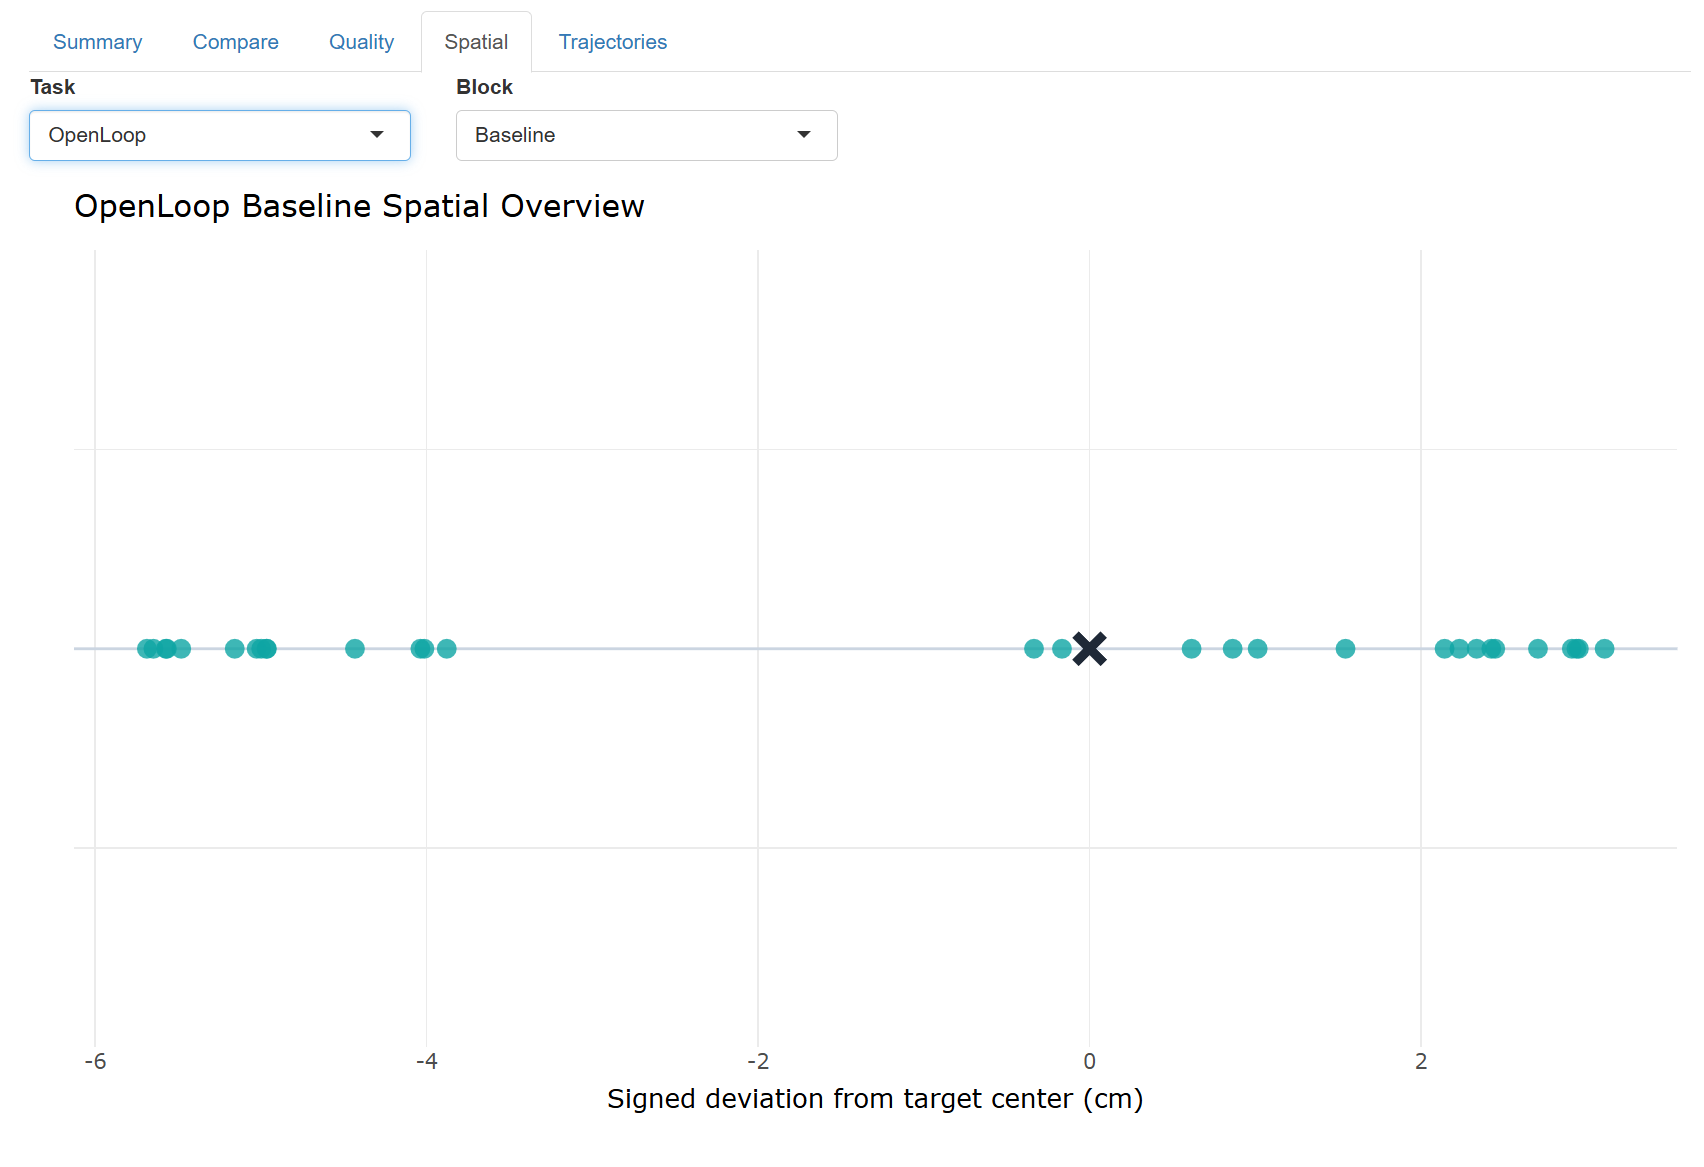
\includegraphics[width=\linewidth]{img/3_Implementation/Spatial3.png}
    \end{minipage}
    \caption{Measurement-task examples from the Spatial tab. Left: Line Bisection baseline responses plotted along the task-relevant horizontal axis, with the cross marking the true midpoint of the displayed line. Right: Open-Loop baseline responses plotted along the same signed horizontal-error axis, with the cross marking the intended target centre. Unlike the exposure view, these plots collapse the response to the left/right dimension that defines the measurement task. The purpose is to expose spatial bias directly rather than only through aggregate trial statistics.}
    \label{fig:rshiny-spatial-measurement}
\end{figure}

\subsubsection{Trajectory View}

The Trajectories tab is the most detailed view in the dashboard, but it deliberately behaves differently for Exposure and for the measurement tasks. Exposure produces a dense sequence of samples within each target-acquisition attempt, so the tab can reconstruct the projected approach path on the target plane, break the visible response window into acceleration, deceleration, and hover, and then inspect how final error evolves across attempts. Open-Loop Pointing and Line Bisection do not always benefit from the same path view, so for those tasks the tab instead becomes a trial-by-trial inspection tool that overlays baseline and post and shows both signed response values and absolute error.

\begin{figure}[H]
    \centering
    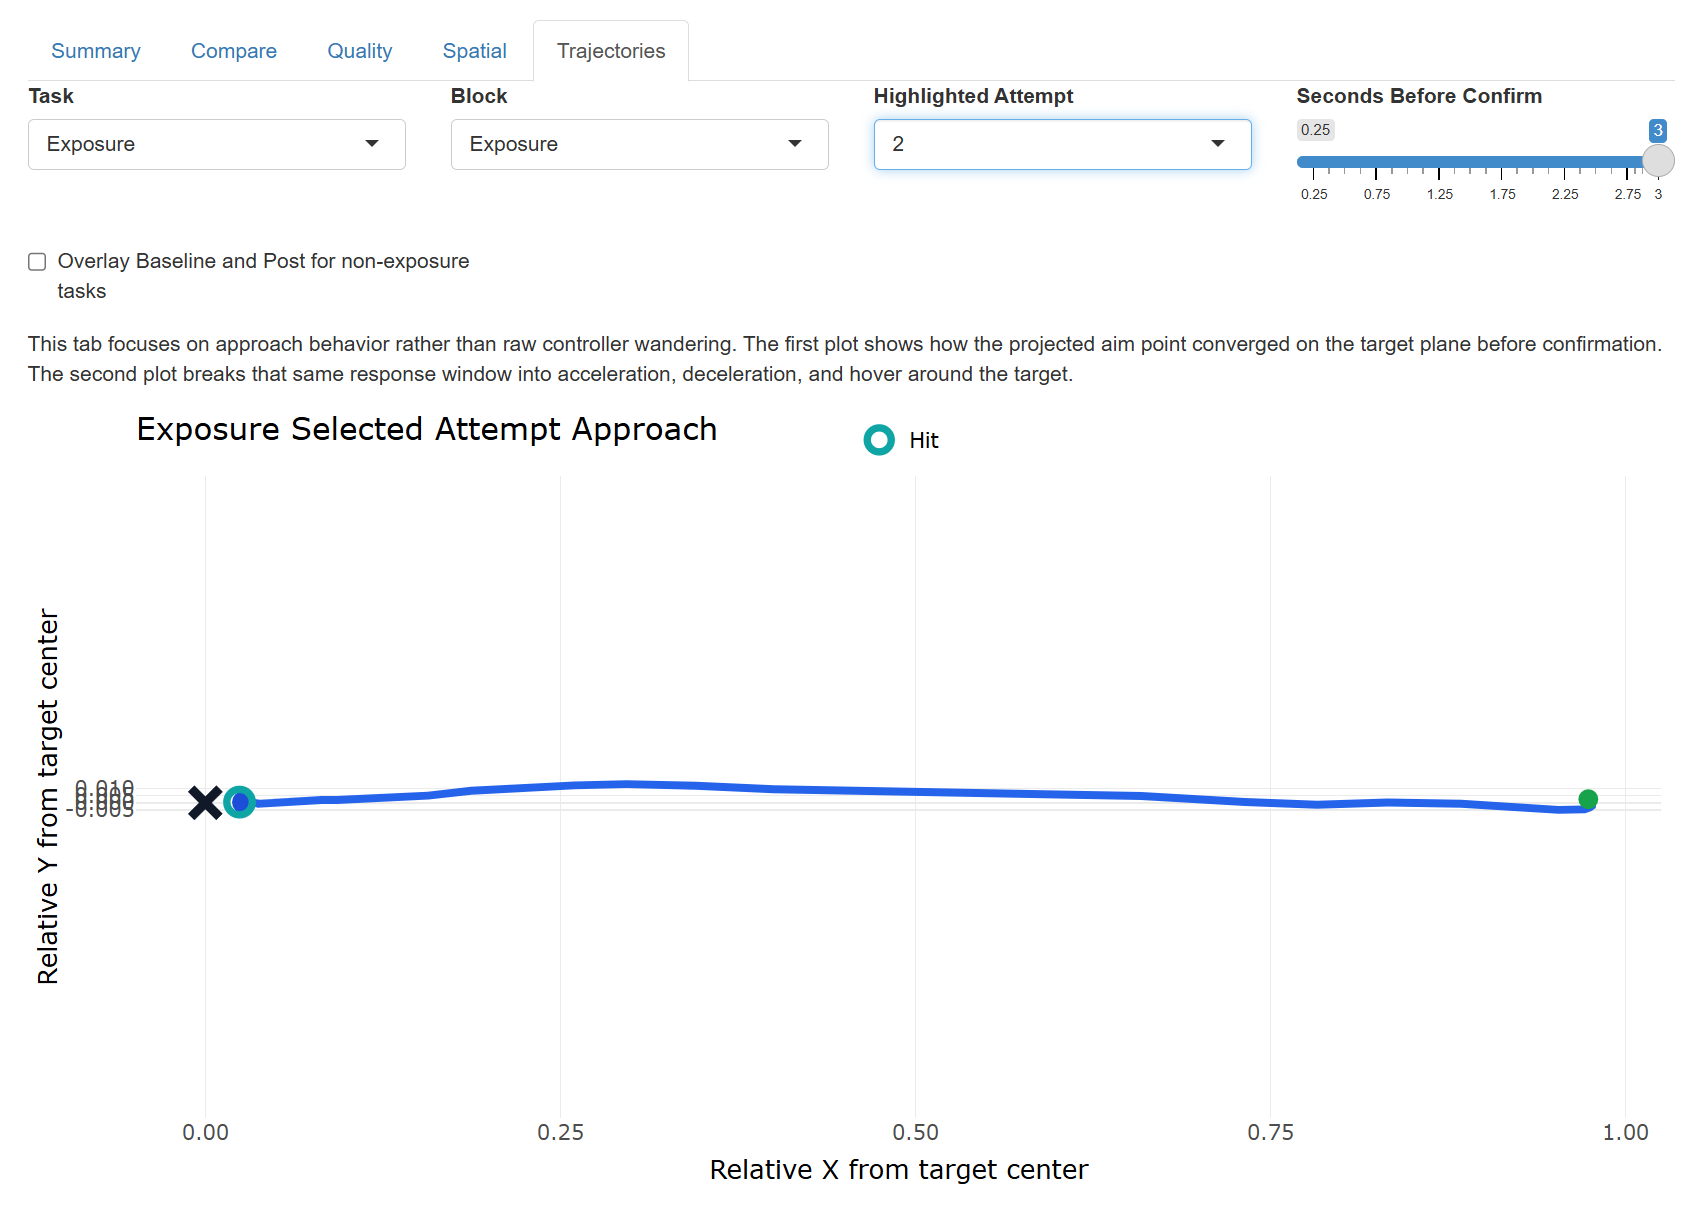
\includegraphics[width=0.98\linewidth]{img/3_Implementation/Trajectory1.png}\par\medskip
    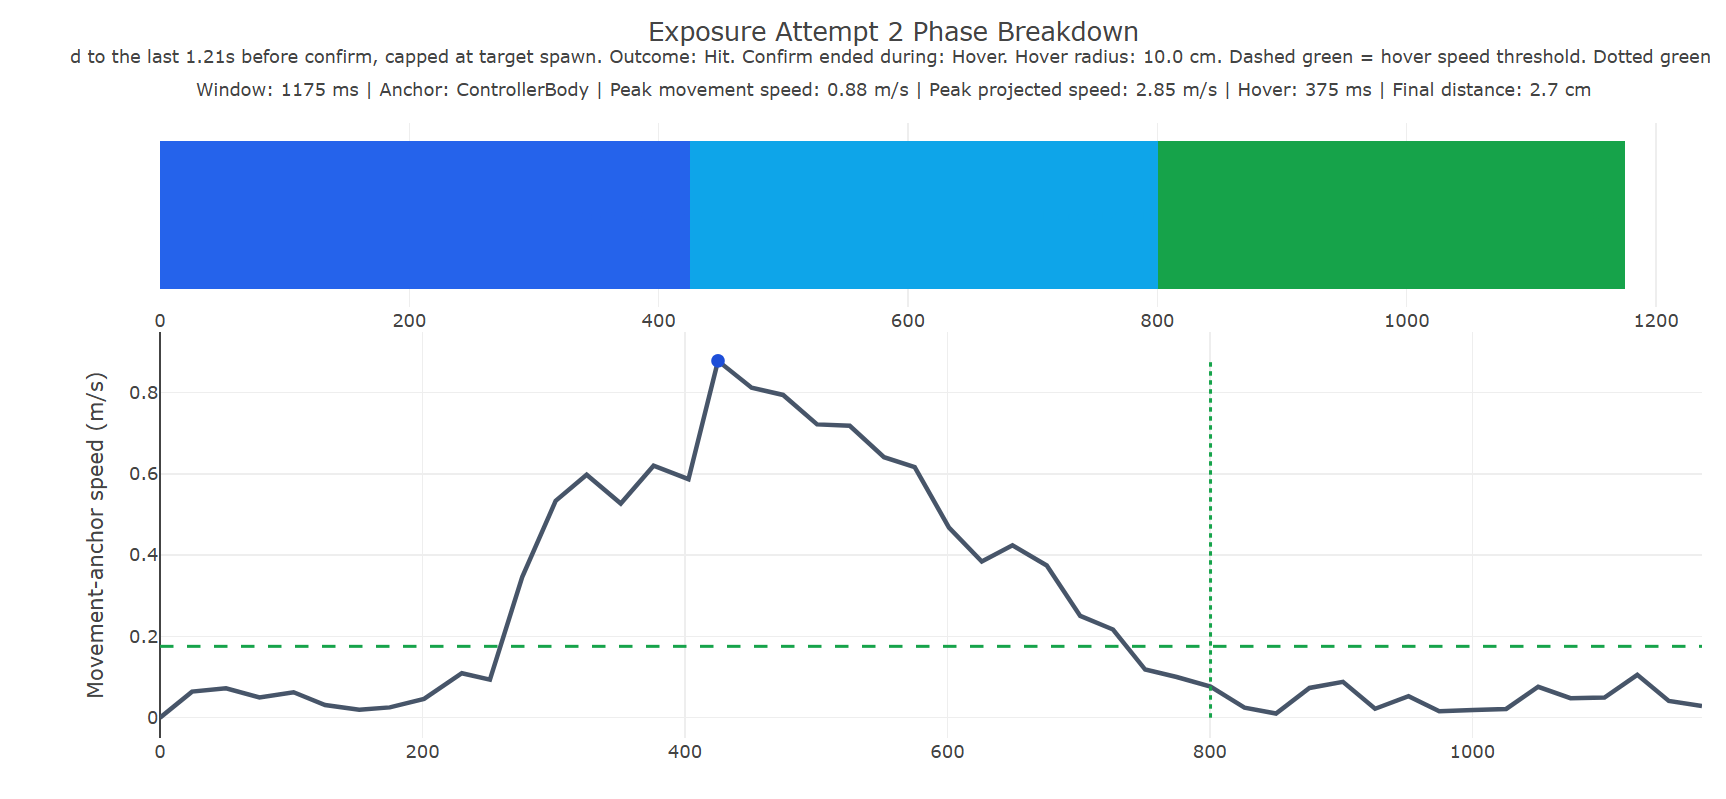
\includegraphics[width=0.98\linewidth]{img/3_Implementation/Trajectory2.png}
    \caption{Exposure-specific views from the Trajectories tab. The upper screenshot shows one selected attempt projected onto the target plane: the cross marks target center, the blue curve shows the projected aim path inside the selected time window, the green point marks the start of the visible path, the blue endpoint marks the final projected pointer, and the hollow circle marks the registered hit position. The lower screenshot breaks that same attempt into acceleration, deceleration, and hover, and plots the associated speed profile with a hover threshold and hover onset marker. Together, these views turn the sampled exposure window into an interpretable description of how the participant approached and stabilized on the target.}
    \label{fig:rshiny-trajectories-exposure}
\end{figure}

\begin{figure}[H]
    \centering
    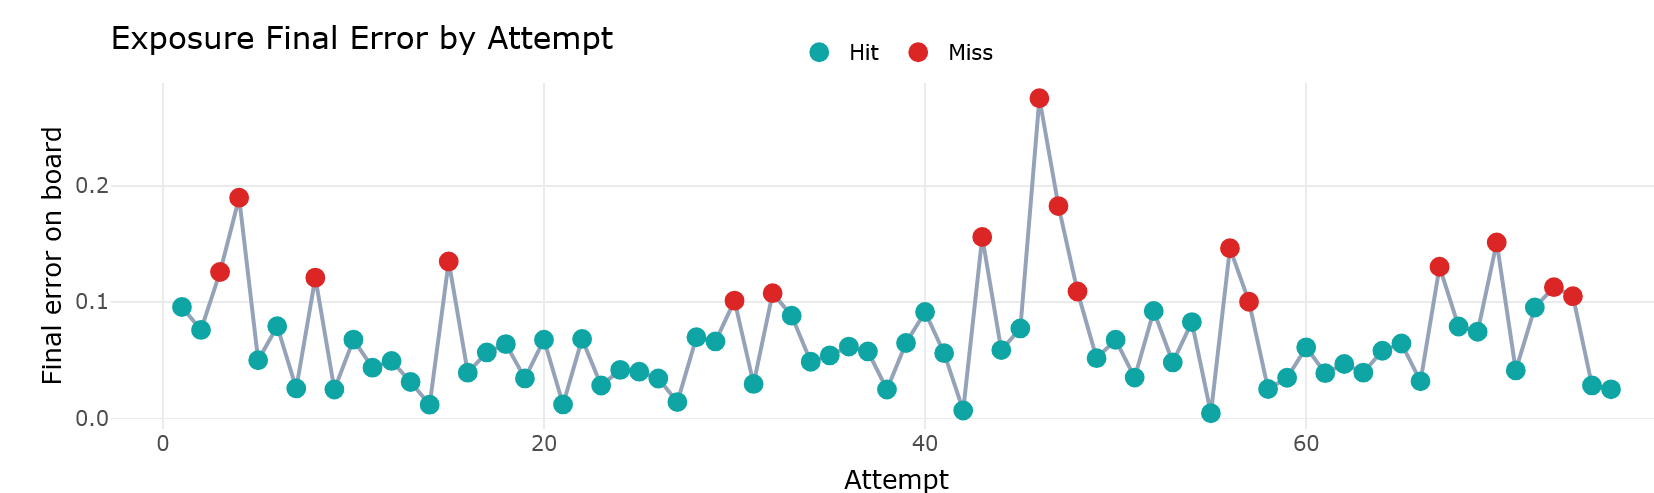
\includegraphics[width=0.98\linewidth]{img/3_Implementation/Trajectory5.png}
    \caption{Exposure final error by attempt. This plot complements the selected-attempt trajectory view by showing how the final board error evolved across the whole exposure block, while preserving the distinction between hits and misses. It is therefore useful for seeing whether one unusual attempt is isolated or part of a broader pattern of poor target acquisition.}
    \label{fig:rshiny-trajectories-exposure-error}
\end{figure}

\begin{figure}[H]
    \centering
    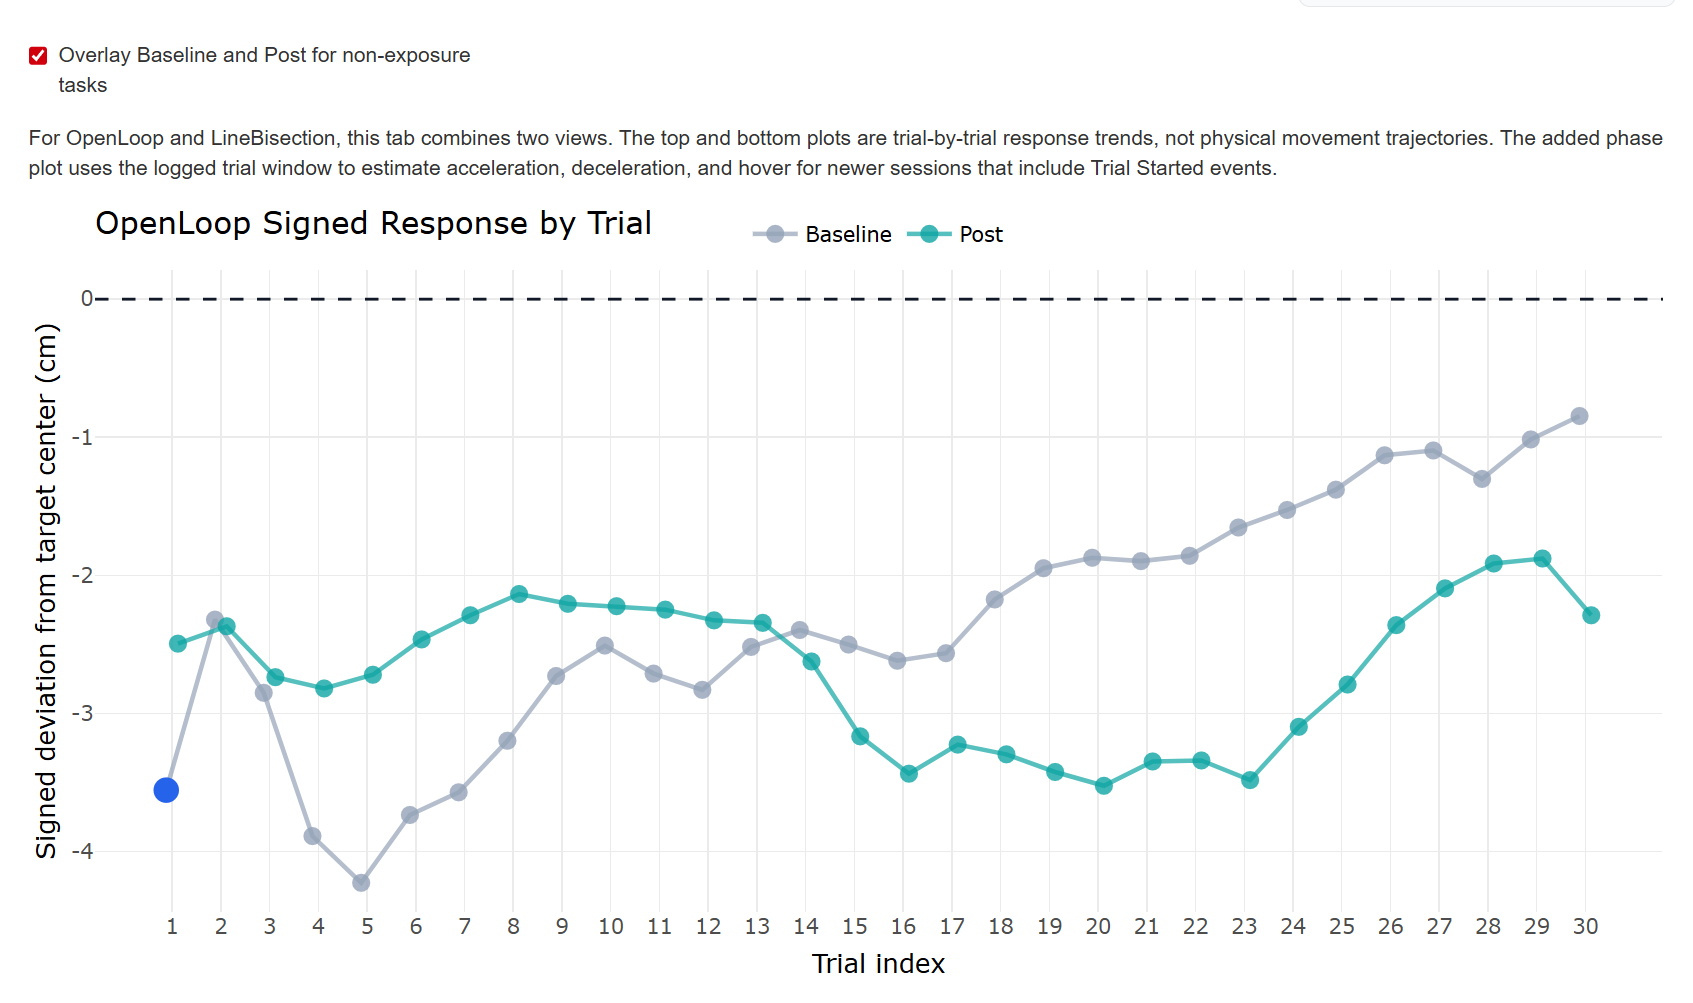
\includegraphics[width=0.98\linewidth]{img/3_Implementation/Trajectory3.png}\par\medskip
    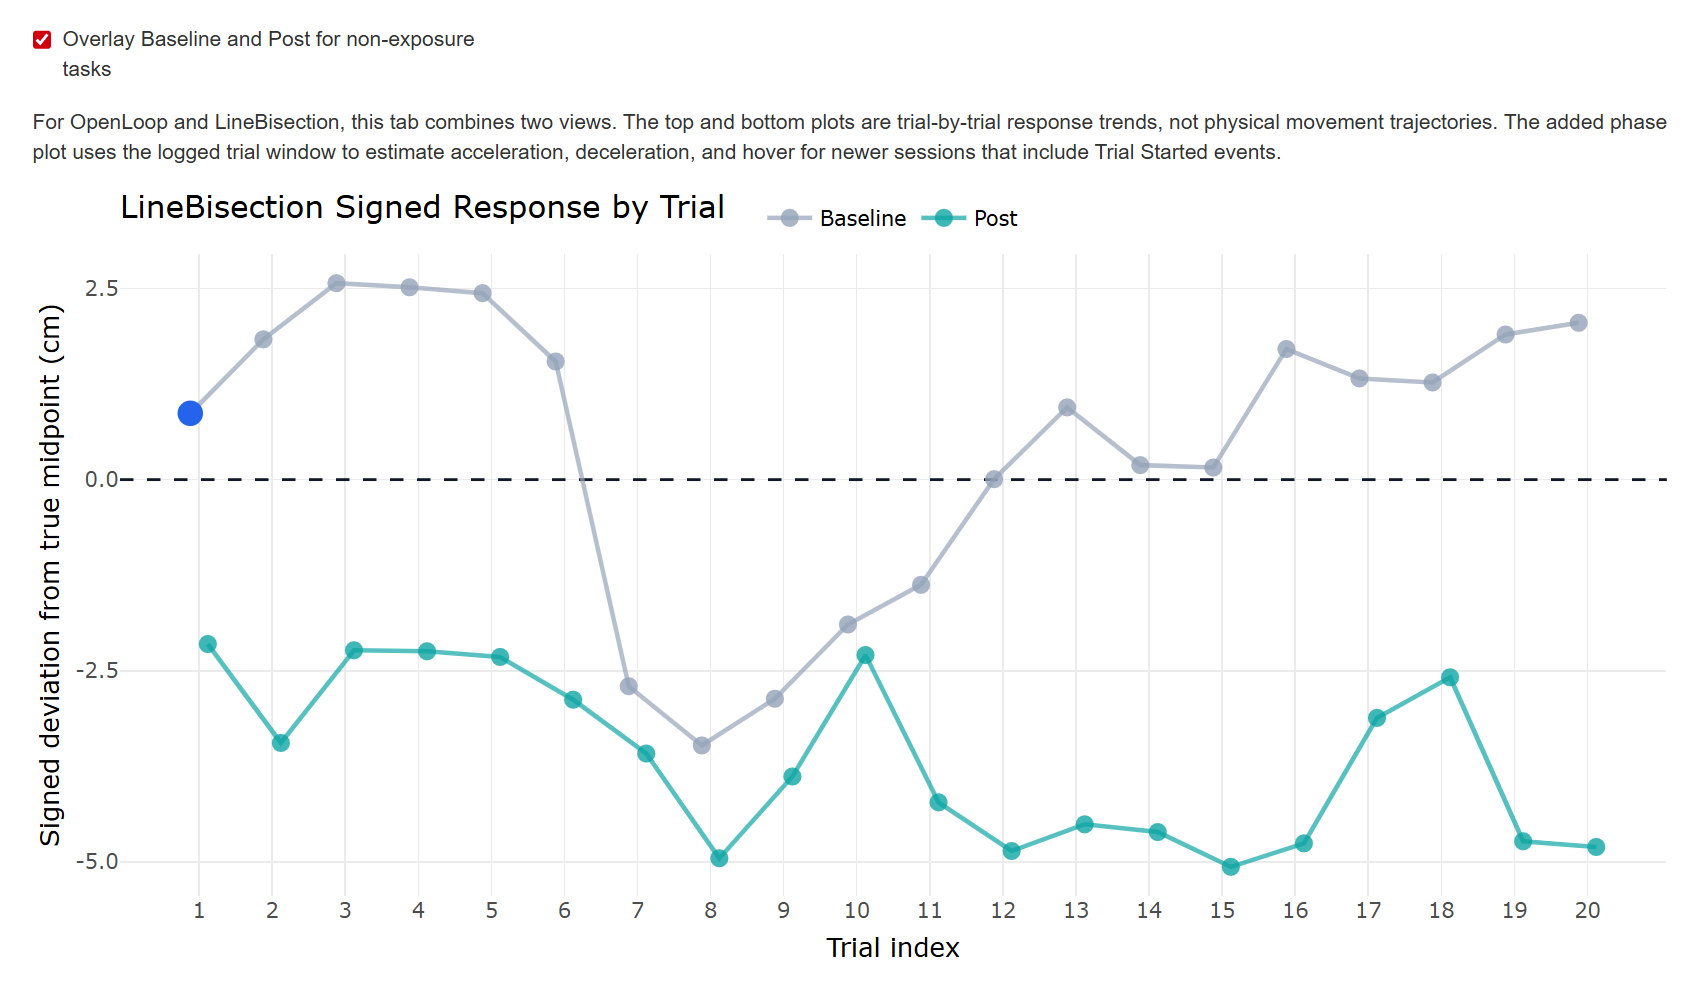
\includegraphics[width=0.98\linewidth]{img/3_Implementation/Trajectory4.png}
    \caption{Signed-response overlays for non-exposure tasks. The upper screenshot shows Open-Loop baseline and post responses overlaid by trial index, and the lower screenshot shows the same idea for Line Bisection. The dashed horizontal line is the ideal centre, and the overlay option shifts baseline and post slightly apart at the same index so both blocks remain readable. In other words, this use of the Trajectories tab is not about raw hand motion in 3D space, but about how signed responses changed between baseline and post across the ordered trial sequence.}
    \label{fig:rshiny-trajectories-measurement-signed}
\end{figure}

\begin{figure}[H]
    \centering
    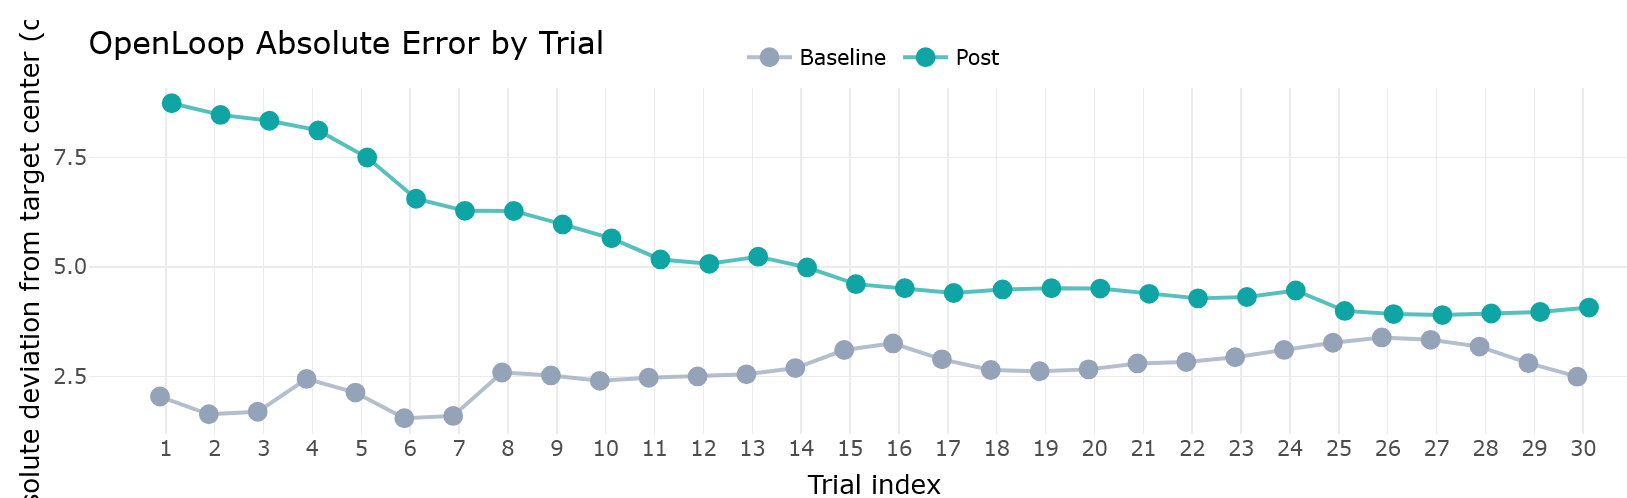
\includegraphics[width=0.98\linewidth]{img/3_Implementation/Trajectory6.png}\par\medskip
    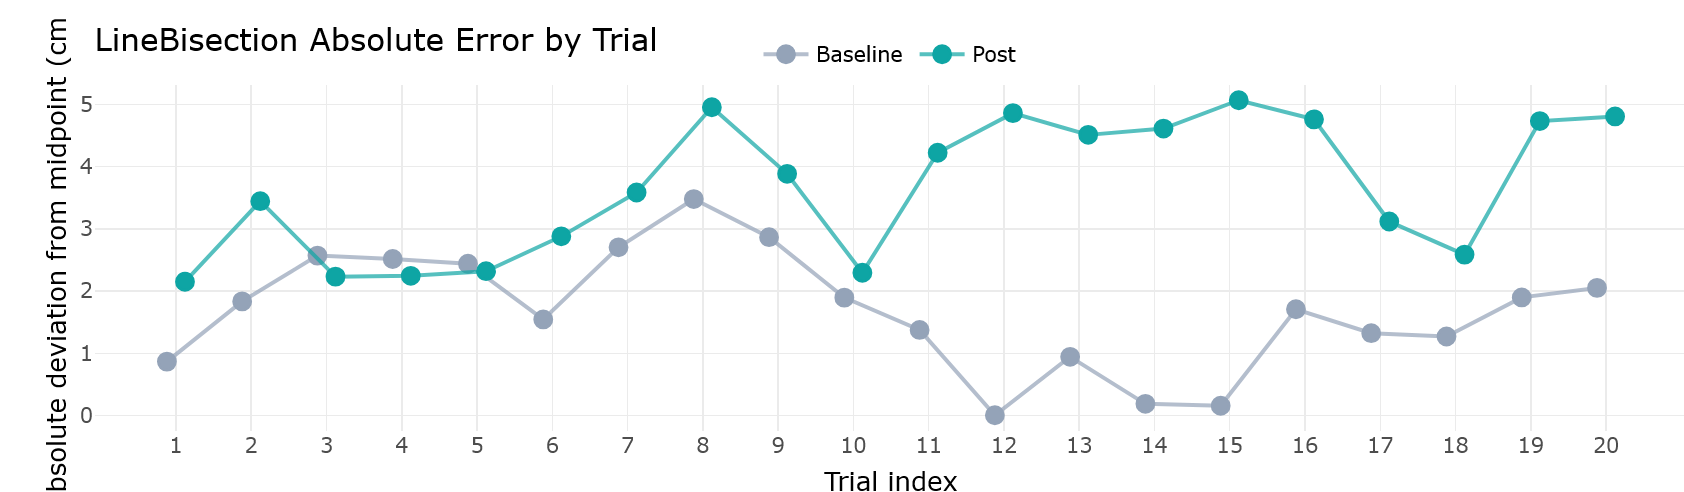
\includegraphics[width=0.98\linewidth]{img/3_Implementation/Trajectory7.png}
    \caption{Absolute-error overlays for non-exposure tasks. The upper screenshot shows Open-Loop absolute deviation from target center by trial, and the lower screenshot shows Line Bisection absolute deviation from the true midpoint by trial, each with baseline and post plotted together. These plots complement the signed-response overlays by showing whether the participant ended closer to or farther from the intended location regardless of left/right direction.}
    \label{fig:rshiny-trajectories-measurement-absolute}
\end{figure}

Taken together, these tabs make the RShiny layer more than a plotting add-on. The same session can be read as an aftereffect summary, a participant-level module profile, a condition comparison, a quality check, a spatial bias pattern, or a movement/response trace depending on which analytical question is being asked. This layer therefore matters because the prototype was built for later inspection as well as runtime use: the Unity side writes the session files, and the dashboard turns those files into a form that can be browsed, compared, and interpreted without manual handling of multiple CSV collections.

\subsection{Script Inventory}
\label{subsec:implementation-script-inventory}

Table~\ref{tab:pegfg-script-inventory} gives a compact overview of the project-specific scripts and their main role in the implemented architecture.

\begin{table}[H]
    \centering
    \footnotesize
    \setlength{\tabcolsep}{5pt}
    \renewcommand{\arraystretch}{1.16}
    \begin{tabularx}{\linewidth}{|
        >{\raggedright\arraybackslash}p{0.27\linewidth}|
        >{\raggedright\arraybackslash}p{0.18\linewidth}|
        X|
    }
        \hline
        \textbf{Script} & \textbf{Layer} & \textbf{Primary responsibility} \\
        \hline
        \texttt{SandboxRunner.cs} & Runtime orchestration & Coordinates calibration, input normalization, confirmation rules, effect selection, and progression between baseline, exposure, and post-exposure blocks. \\
        \hline
        \texttt{PrismCore.cs} & Effect layer & Defines the effect abstractions and the concrete \emph{none}, \emph{translation}, \emph{rotation}, and \emph{skew} transforms used during the exposure phase. \\
        \hline
        \texttt{OpenLoopPointingTask.cs} & Task layer & Implements the single-target measurement task and computes signed endpoint error relative to the intended target center. \\
        \hline
        \texttt{LineBisectionTask.cs} & Task layer & Implements midpoint estimation on a displayed line and computes signed deviation from the true midpoint. \\
        \hline
        \texttt{LandmarkTask.cs} & Task layer & Implements the comparative left/right judgment task and computes correctness and response bias. \\
        \hline
        \texttt{ExposureTask.cs} & Task layer & Implements the repeated target-acquisition phase under perturbation, including target selection, hit/miss classification, and exposure completion. \\
        \hline
        \texttt{HandDwellProgressBar.cs} & UI / feedback & Visualizes loading and transition timing between interactions. Despite the script name, the final evaluation used opposite-hand trigger confirmation rather than dwell confirmation. \\
        \hline
        \texttt{RoundedRectGraphic.cs} & UI support & Generates rounded rectangle meshes used by the custom progress-bar interface. \\
        \hline
        \texttt{PrismExperimentLogger.cs} & Logging & Writes metadata, event rows, block summaries, and aftereffect summaries in a format aligned with the experiment structure. \\
        \hline
        \texttt{PrismSampleLogger.cs} & Logging & Writes regular sample snapshots of pointer, head, controller, and movement-anchor state for later trajectory analysis. \\
        \hline
        \texttt{app.R} & Analysis & Loads completed sessions and visualizes them as summary, compare, participant, quality, spatial, and trajectory views in the local RShiny dashboard. \\
        \hline
    \end{tabularx}
    \caption{Project-specific script inventory for the prototype. The table groups the files by architectural role rather than by folder location and makes the runtime, task, feedback, logging, and analysis responsibilities easier to distinguish.}
    \label{tab:pegfg-script-inventory}
\end{table}

\subsection{From Runtime to Analysis}
\label{subsec:implementation-overall-workflow}

Taken together, the implementation follows one layered workflow. \texttt{SandboxRunner.cs} coordinates calibration, input handling, and block progression; the task scripts run the individual baseline, exposure, and post-exposure procedures; the logging layer turns the run into stable CSV collections; and \texttt{app.R} rebuilds those collections into analysis views. The result is a prototype in which participant interaction, stored data, and later inspection are all part of the same workflow.
